\documentclass[a4paper]{ctexart}
\usepackage{xeCJK}
\usepackage{times}
\usepackage{setspace}
\usepackage{fancyhdr}
\usepackage{graphicx}
\usepackage{wrapfig}
\usepackage{array}
\usepackage{fontspec,xunicode,xltxtra}
\usepackage{titlesec}
\usepackage{titletoc}
\usepackage[titletoc]{appendix}
\usepackage[top=29mm,bottom=29mm,left=31.8mm,right=31.8mm]{geometry}
\usepackage{enumerate}
\usepackage{caption,subcaption}
\usepackage{amsmath,bm}
\usepackage{cite}
\setmainfont{Times New Roman}
\setCJKmainfont[BoldFont={Songti SC Bold}]{SimSun}
\setCJKfamilyfont{heiti}{SimHei}
\renewcommand{\heiti}{\CJKfamily{heiti}\fontspec{Times New Roman}}

\newcommand{\mycaptionfont}{\heiti\zihao{5}}
\captionsetup[figure]{name={\mycaptionfont 图},labelsep=period}
\captionsetup[subfigure]{name={\mycaptionfont},labelsep=period}
\renewcommand{\captionfont}{\mycaptionfont}
\renewcommand{\captionlabelfont}{\mycaptionfont}

\newcommand{\outwfour}{0.23\textwidth}
\newcommand{\outwthree}{0.3\textwidth}
\newcommand{\outwtwo}{0.4\textwidth}

\ctexset {
	section = {
		number = \chinese{section},
		format = \zihao{4}\bfseries,
		},
	subsection = {
		number = \arabic{section}.\arabic{subsection},
		format = \zihao{-4}\bfseries,
		}
}


\setlength\parskip{.5\baselineskip}
\fancypagestyle{plain}{\pagestyle{fancy}}%改变章节首页页眉
\pagestyle{fancy}
\lhead{}
\chead{视觉物联网技术实验报告}
\rhead{}
\cfoot{\thepage}

\begin{document}
\begin{titlepage}
	\begin{center}
		
\includegraphics[width=0.9\textwidth]{figure//Njust.png}\\
		\vspace{10mm}
		\textbf{\zihao{2}\kaishu{物联网工程学院}}\\[0.8cm]
		\textbf{\zihao{2}\kaishu{视觉物联网技术实验报告}}\\[3cm]
		\textbf{\zihao{2}\kaishu{实验一~图像处理}}\\[3cm]
		\vspace{\fill}
		\setlength{\extrarowheight}{3mm}
		{\songti\zihao{3}
			\begin{tabular}{rl}
				{\makebox[4\ccwd][s]{班\qquad 级:}} & ~\kaishu 物联1601   \\
				{\makebox[4\ccwd][s]{姓\qquad 名:}} & ~\kaishu 尹达恒     \\
				{\makebox[4\ccwd][s]{学\qquad 号:}} & ~\kaishu 1030616134 \\
				{\makebox[4\ccwd][s]{指导老师:}}    & ~\kaishu 陈莹       \\
			\end{tabular}
		}\\[2cm]
		\vspace{\fill}
		\zihao{4}
		2018\textasciitilde 2019第二学期\\
		2019年3月28日
	\end{center}
\end{titlepage}


\begin{spacing}{1.35}
	\zihao{-4}
	\section{实验名称:图像处理}
	\begin{table}[htbp]
		\zihao{4}
		\begin{tabular}{lll}
			班级:物联网1601 & 姓名:尹达恒                                 & 学号:1030616134 \\
			                 &                                              &                  \\
			时间:2019/3/28  & \multicolumn{2}{l}{地点:物联网工程学院D416}                    \\
		\end{tabular}
	\end{table}
	\section{实验目的}
	\begin{enumerate}[1、]
		\item 使学生通过分析图片,采用合适的图像增强方法获得较为清晰的图片,进而加强对各 种图像增强方法的了解;
		\item 能够利用二值形态学消除干扰,获得目标图像;
		\item 能够了解各种图像增强方法中参数的选择对处理结果的影响;
		\item 完成规定图像的处理并要求正确评价处理结果,能够从理论上作出合理的解释。
	\end{enumerate}
	\section{实验内容}
	\begin{enumerate}[1、]
		\item {\bf 选用合适的图像增强方法}对以下给定图像(图\ref{pic:1}、图\ref{pic:2}、图\ref{pic:3}、图\ref{pic:4})进行增强操作以获取清晰图像;
		      \begin{figure*}[htbp]
			      \centering
			      \begin{minipage}[t]{\outwtwo}
				      \centering
				      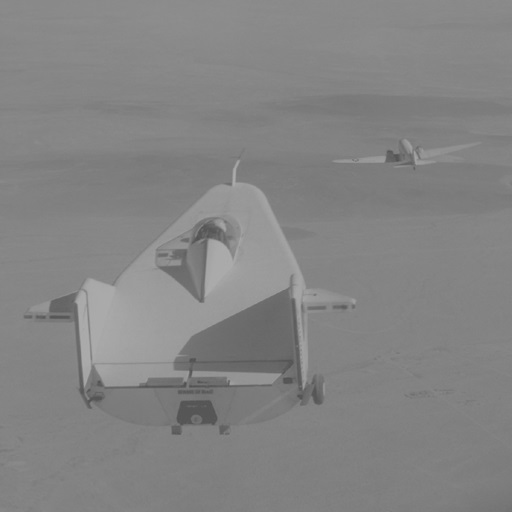
\includegraphics[width=1.4in]{figure//image1.jpg}
				      \caption{}\label{pic:1}
			      \end{minipage}
			      \begin{minipage}[t]{\outwtwo}
				      \centering
				      \includegraphics[width=1.4in]{figure//image2.jpg}
				      \caption{}\label{pic:2}
			      \end{minipage}\\
			      \begin{minipage}[t]{\outwtwo}
				      \centering
				      \includegraphics[width=1.4in]{figure//image3.jpg}
				      \caption{}\label{pic:3}
			      \end{minipage}
			      \begin{minipage}[t]{\outwtwo}
				      \centering
				      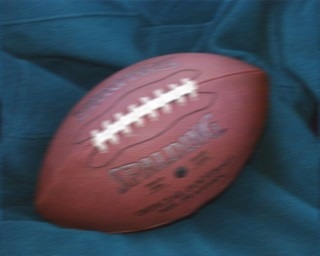
\includegraphics[width=1.4in]{figure//image4.jpg}
				      \caption{}\label{pic:4}
			      \end{minipage}
		      \end{figure*}
		\item 对步骤1处理后的图\ref{pic:3}进行阈值处理,获得二值图像,并对其进行形态学分析,提取 有用信息区域(即只剩下字母和数字区域)。
	\end{enumerate}

	\section{实验步骤}
	\subsection{对图\ref{pic:1}的分析与图像增强}\label{sec:处理1}
	首先使用opencv中的cv2.calcHist()函数绘制图\ref{pic:1}的灰度直方图(图\ref{fig:灰度直方图1})。
	\begin{figure}[htbp]
		\centering
		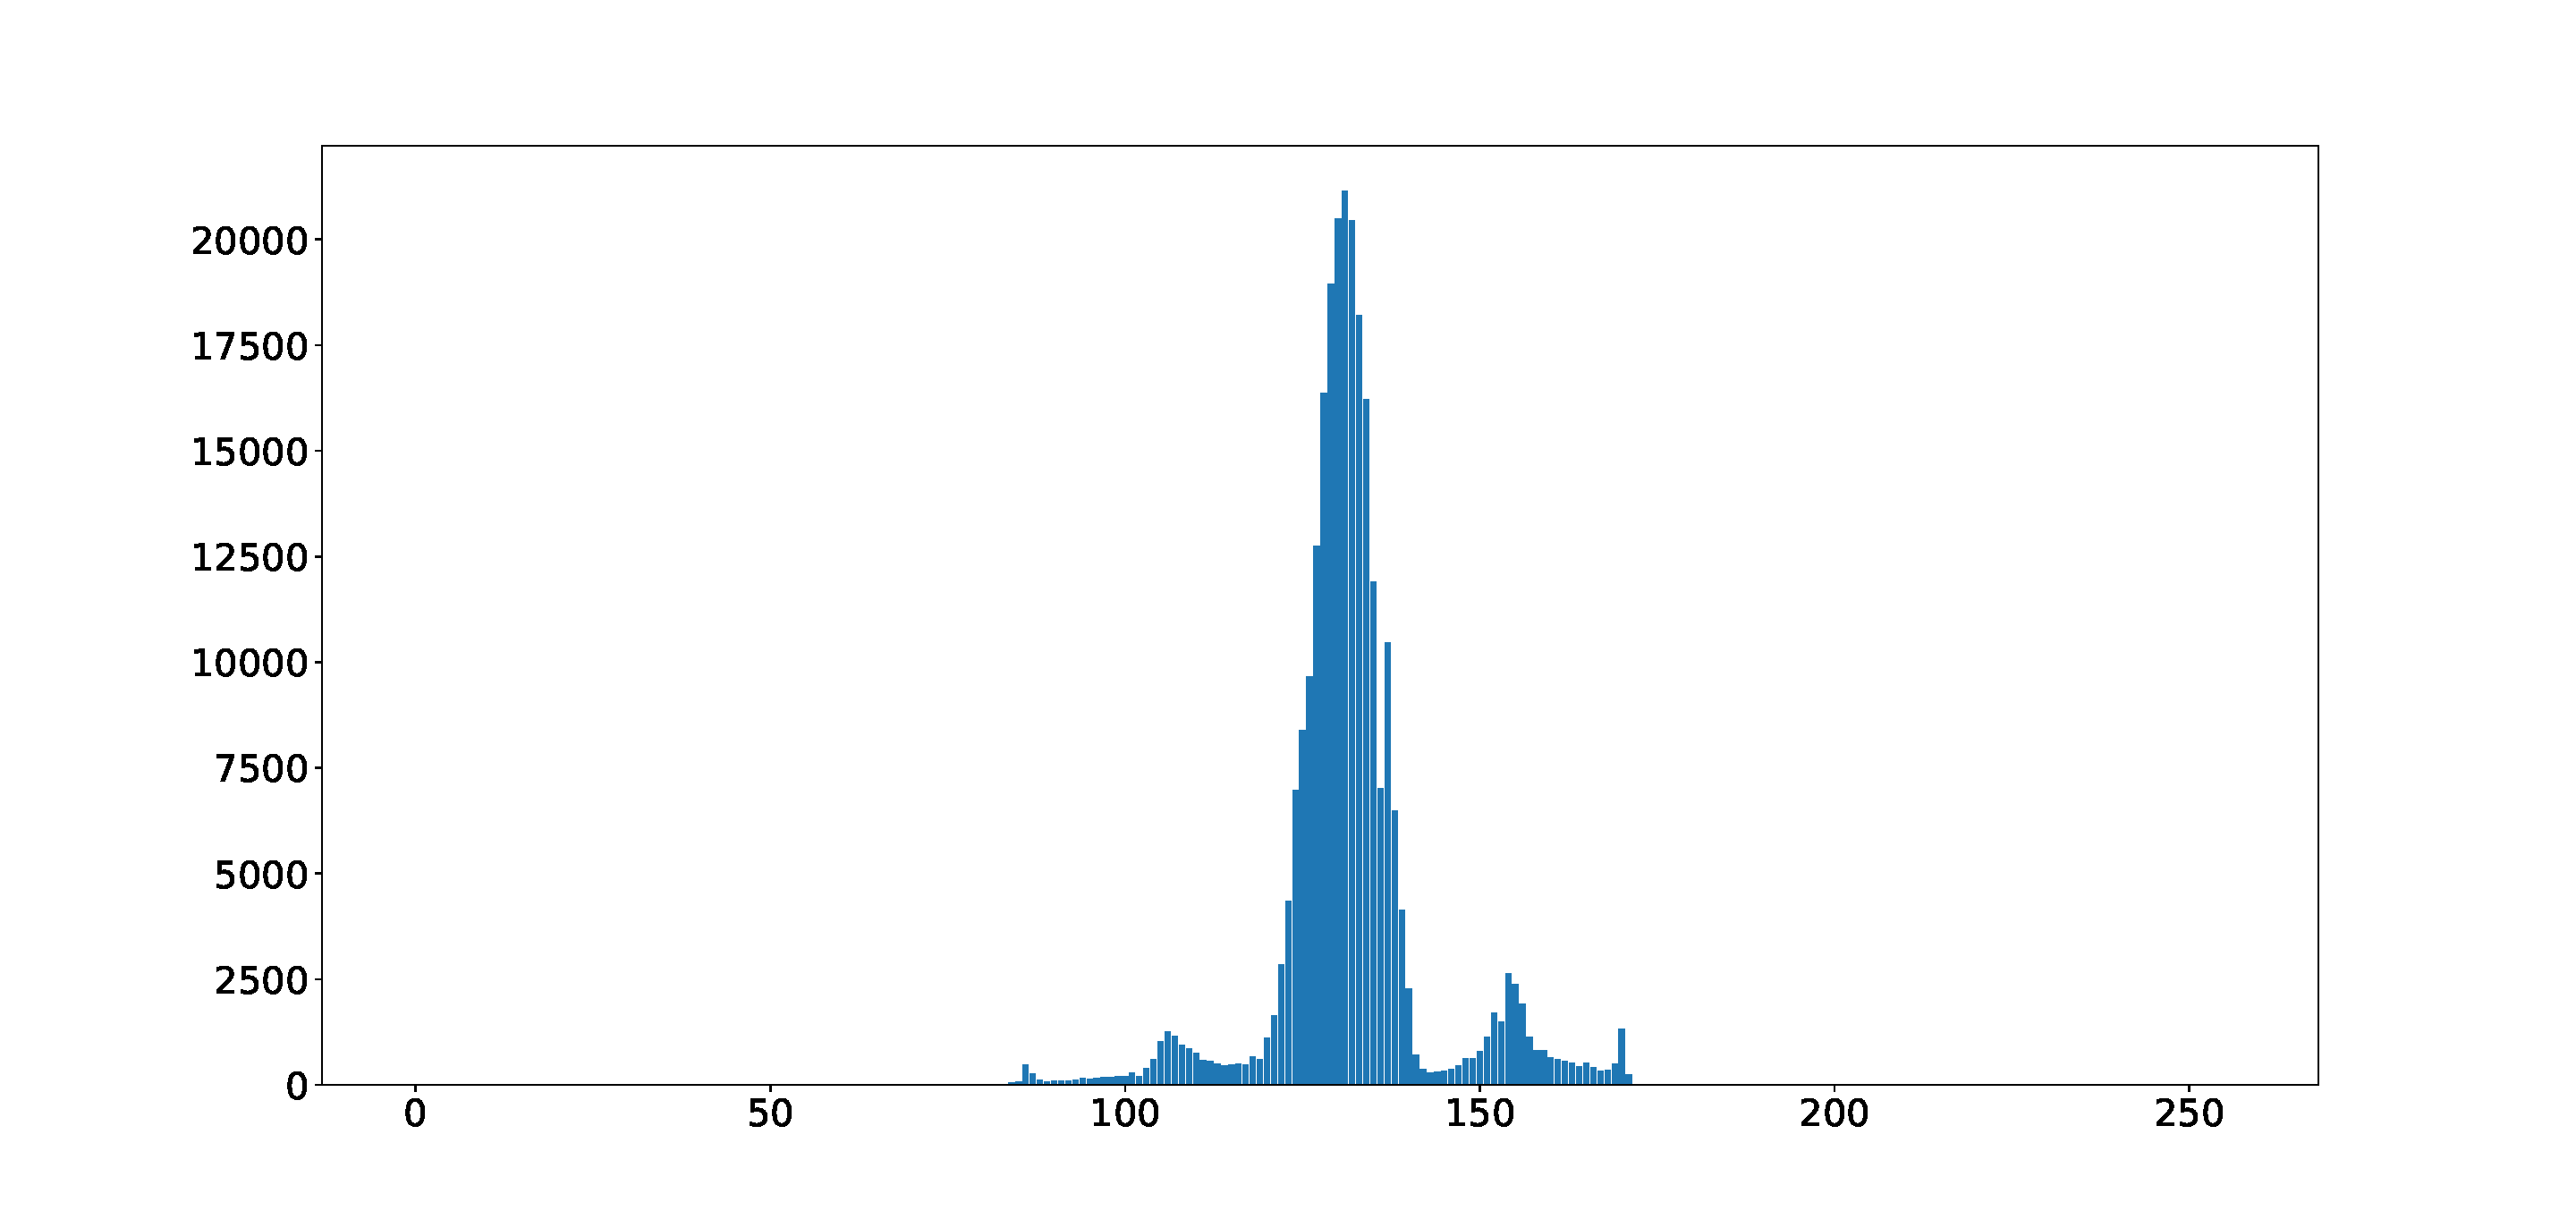
\includegraphics[width=\textwidth]{figure/hist_1.pdf}
		\caption{图\ref{pic:1}的灰度直方图}\label{fig:灰度直方图1}
	\end{figure}
	从灰度直方图中我们可以很明显的看出,图\ref{pic:1}存在灰度分布不均的问题,其大部分像素的灰度值都集中于100$\sim$180之间(灰度值为0$\sim$255),因此首先应该对图像进行直方图均衡化。首先使用标准的直方图均衡化方法cv2.equalizeHist()对图像进行增强,得到均衡化后的图片和直方图如图\ref{fig:标准直方图均衡化}。
	\begin{figure}[htbp]
		\centering
		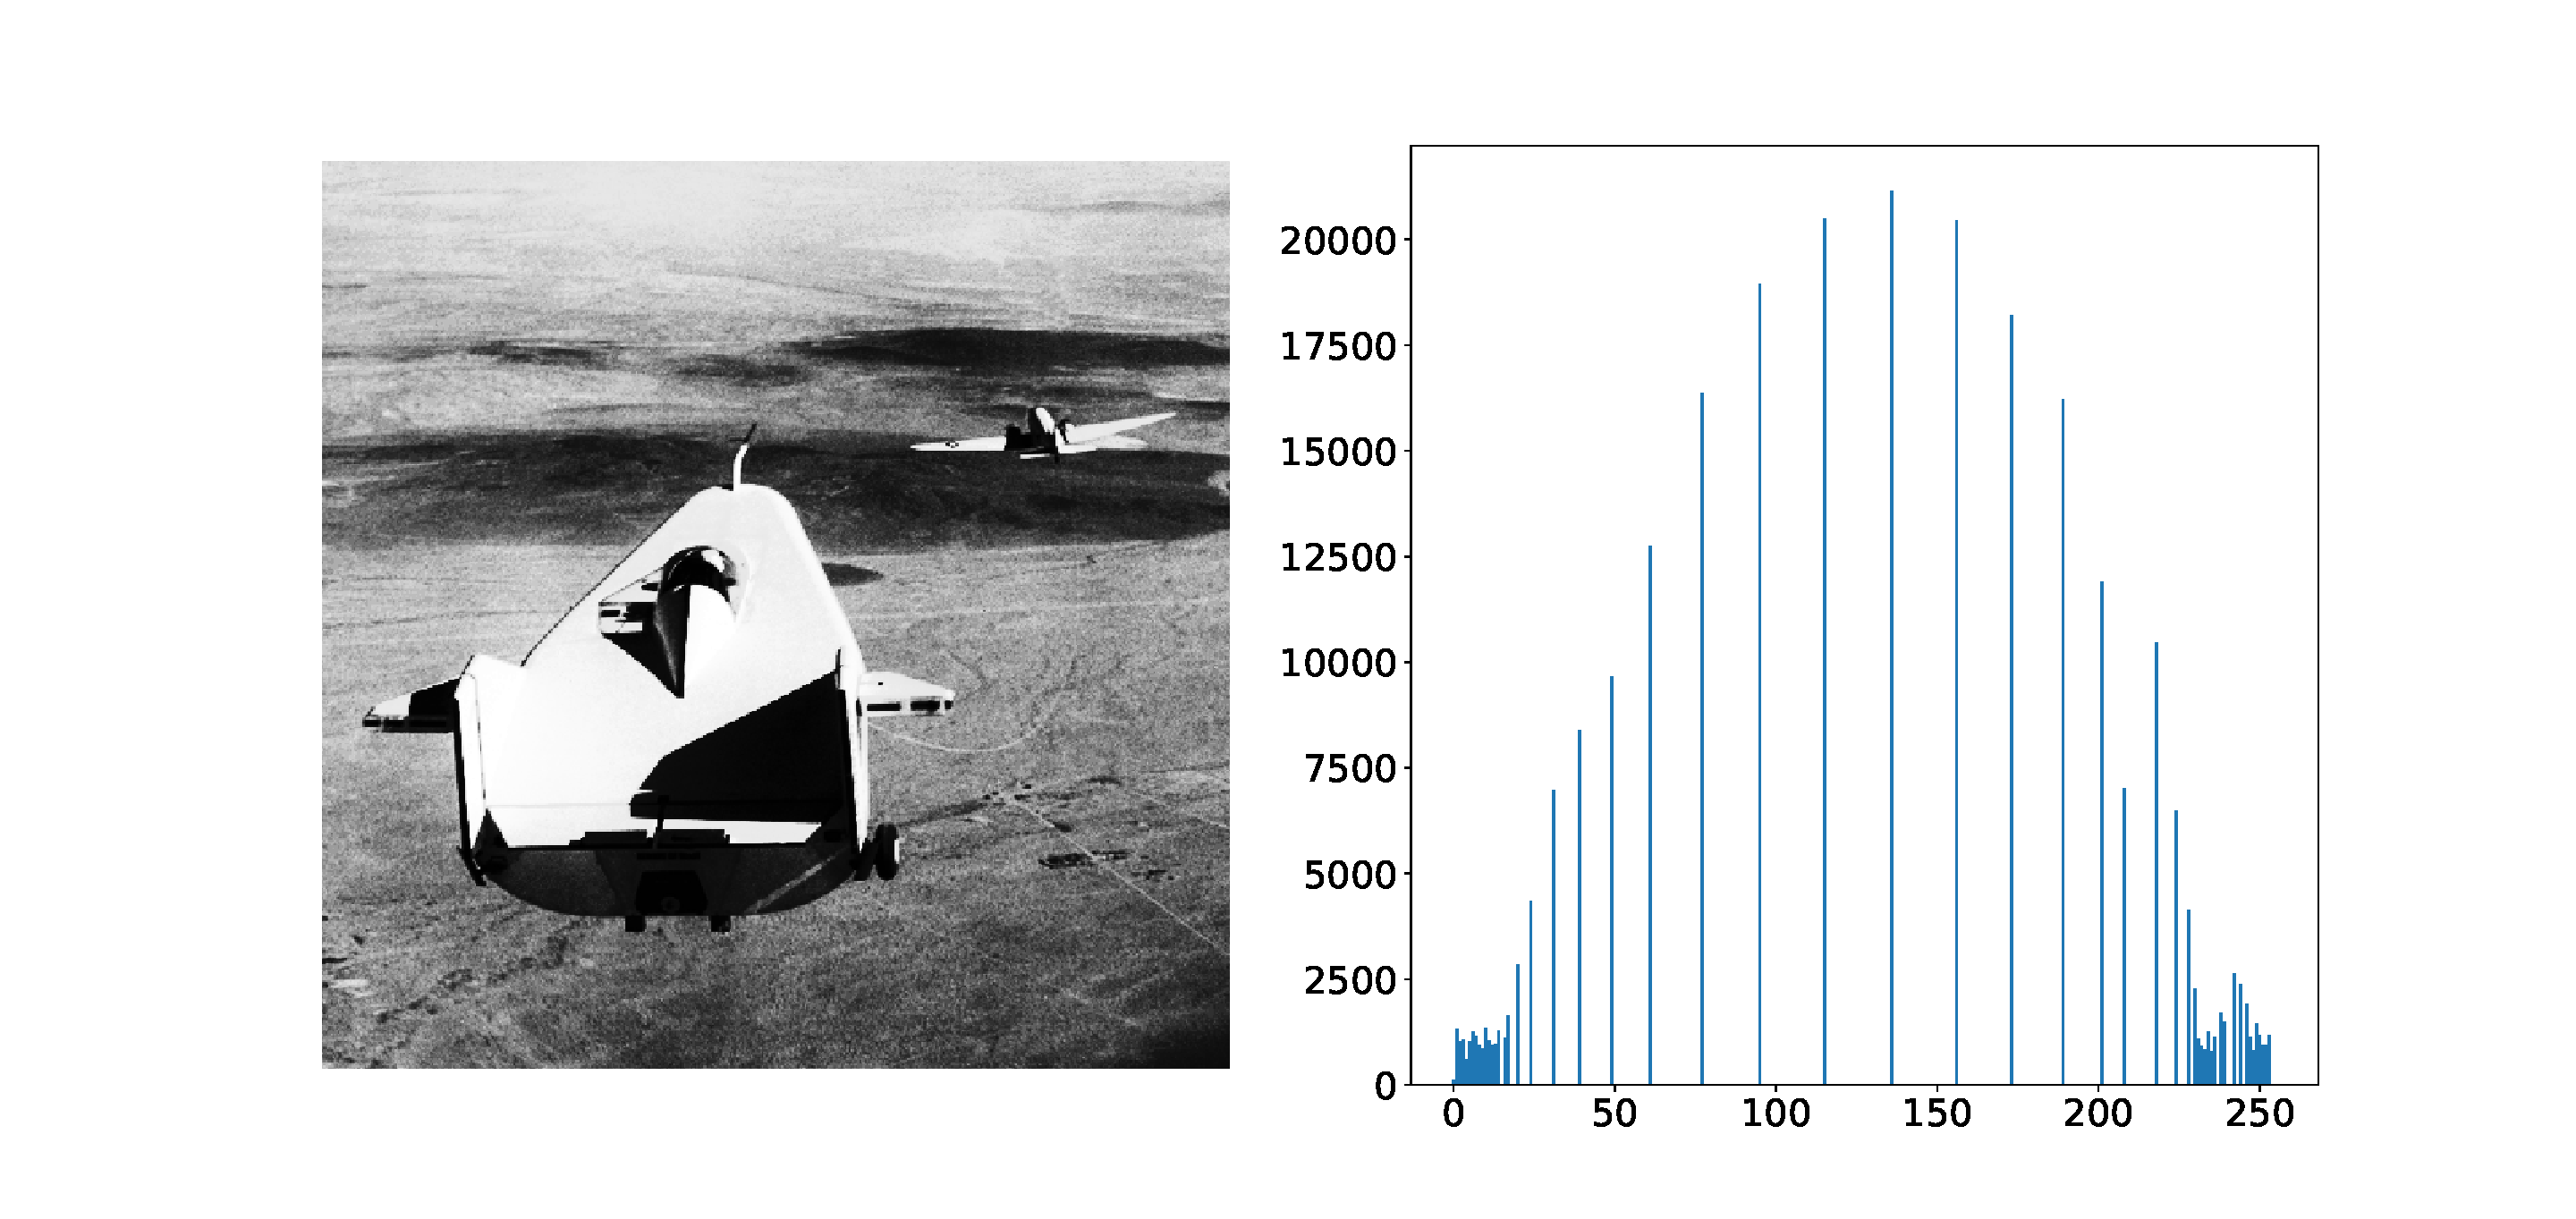
\includegraphics[width=\textwidth]{figure/eqhist_1.pdf}
		\caption{图\ref{pic:1}经过标准直方图均衡化的处理结果}\label{fig:标准直方图均衡化}
	\end{figure}
	从图中可以看出,标准直方图均衡化虽然有效地分散了灰度值分布,但分散后的图像部分区域局部灰度值相差甚远,使得图像的噪声被放大、且对比度过强,图像增强效果不理想。为解决此问题,使用对比度受限的自适应直方图均衡化方法(contrast-limited adapative histogram equalization,CLAHE)\cite{RN150}\cite{RN153}对图像进行均衡化。这里先选用剪切限制(clip limit)为2、滑动窗口(tile grid)为8$\times$8的CLAHE对图像进行处理,得到的图像和直方图如图\ref{fig:CLAHE1}所示。
	\begin{figure}[htbp]
		\centering
		\begin{minipage}[t]{0.351\textwidth}
			\centering
			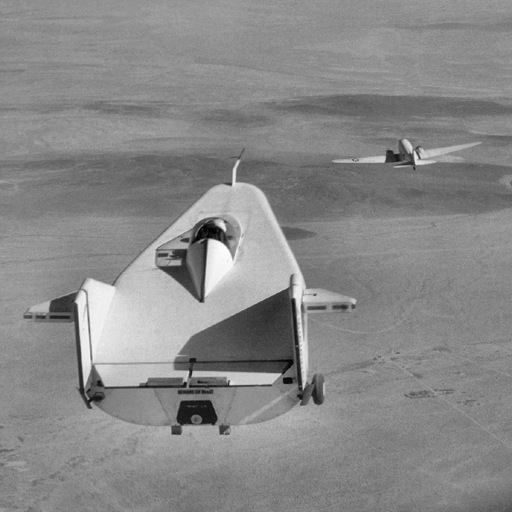
\includegraphics[width=\textwidth]{figure/1_clip_limit_2.png}
		\end{minipage}
		\begin{minipage}[t]{0.44\textwidth}
			\centering
			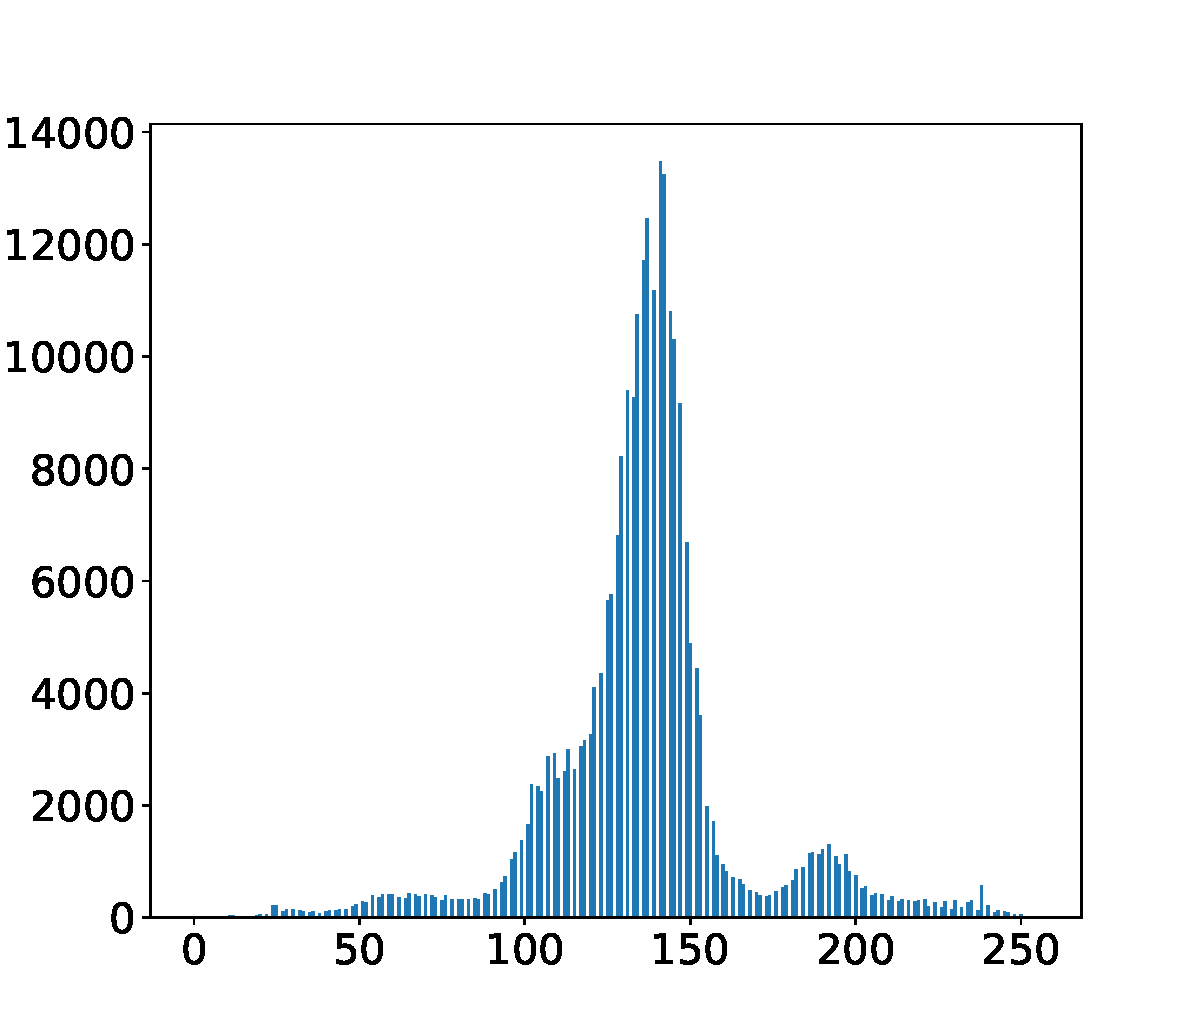
\includegraphics[width=\textwidth]{figure/CLAHEhist_1.pdf}
		\end{minipage}
		\caption{剪切限制为2、滑动窗口边长为8时的CLAHE处理结果}
		\label{fig:CLAHE1}
	\end{figure}
	从图中可以看出,CLAHE虽然不能完全利用图像的灰度域,但是在处理中很好的限制了图像的对比度,处理效果要好于标准的直方图均衡化方法。保持滑动窗口边长不变,分别修改剪切限制、为3、4、5,CLAHE处理结果如图\ref{fig:CLAHE2}。

	\begin{figure}[htbp]
		\centering
		\begin{subfigure}[t]{\outwfour}
			\centering
			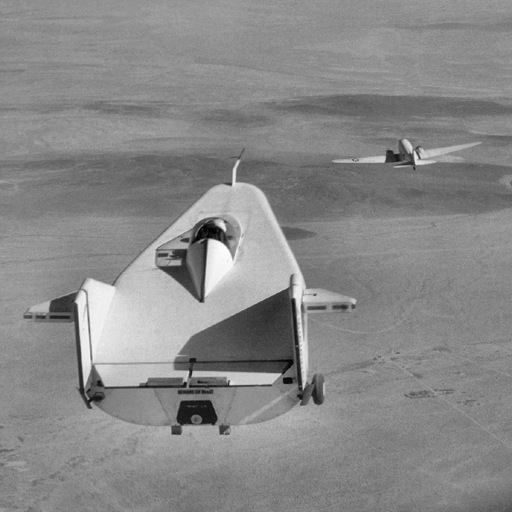
\includegraphics[width=\textwidth]{figure/1_clip_limit_2.png}
			\caption{剪切限制=2}
		\end{subfigure}
		\begin{subfigure}[t]{\outwfour}
			\centering
			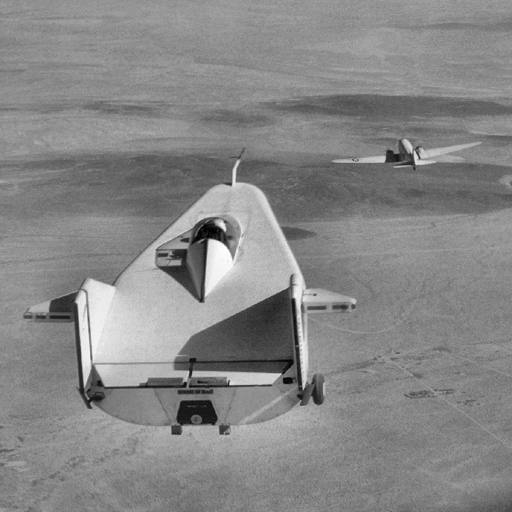
\includegraphics[width=\textwidth]{figure/1_clip_limit_3.png}
			\caption{剪切限制=3}
		\end{subfigure}
		\begin{subfigure}[t]{\outwfour}
			\centering
			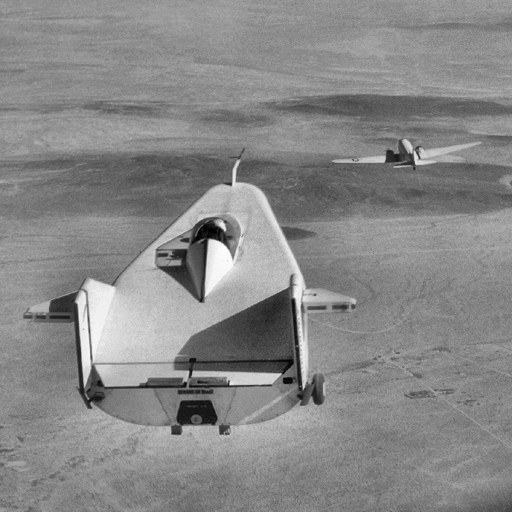
\includegraphics[width=\textwidth]{figure/1_clip_limit_4.png}
			\caption{剪切限制=4}
		\end{subfigure}
		\begin{subfigure}[t]{\outwfour}
			\centering
			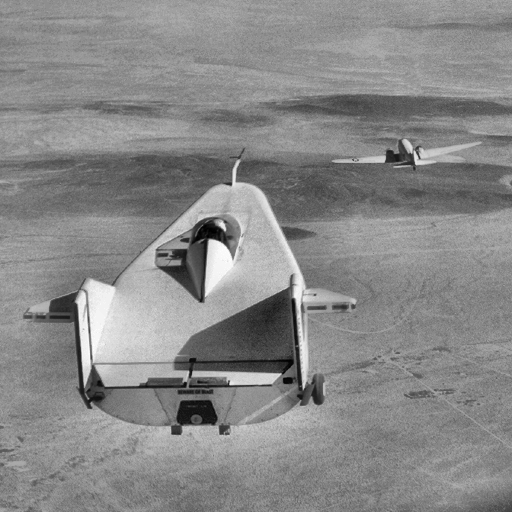
\includegraphics[width=\textwidth]{figure/1_clip_limit_5.png}
			\caption{剪切限制=5}
		\end{subfigure}
		\caption{剪切限制为2、3、4、5、滑动窗口边长为8时的CLAHE处理结果}
		\label{fig:CLAHE2}
	\end{figure}
	可以看出,随着剪切限制的增大,图像的对比度在增强的同时,其噪声也被一并增强了。

	从图\ref{fig:CLAHE2}中选择处理效果较好的CLAHE处理结果进行进一步调整。这里选择处理结果的对比度和噪声适中的剪切限制为2,调节其滑动窗口边长为4、8、12、16,CLAHE处理结果如图\ref{fig:CLAHE3}。
	\begin{figure}[htbp]
		\centering
		\begin{subfigure}[t]{\outwfour}
			\centering
			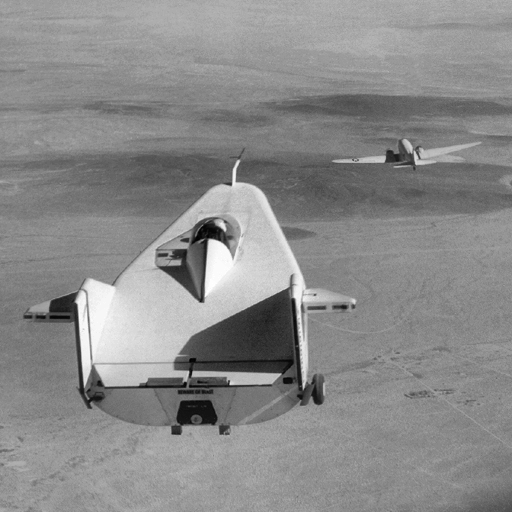
\includegraphics[width=\textwidth]{figure/1_tile_grid_size_4.png}
			\caption{滑动窗口边长=4}
		\end{subfigure}
		\begin{subfigure}[t]{\outwfour}
			\centering
			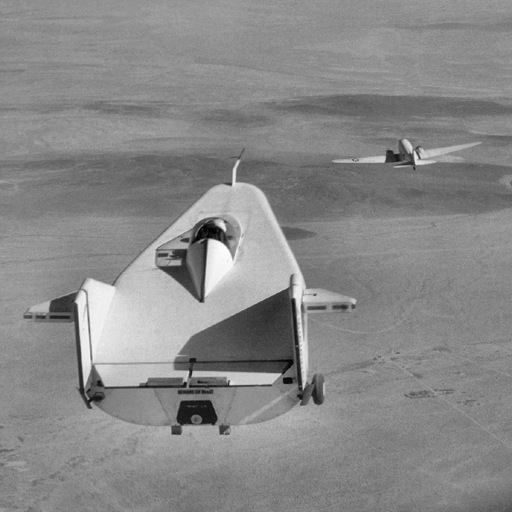
\includegraphics[width=\textwidth]{figure/1_tile_grid_size_8.png}
			\caption{滑动窗口边长=8}
		\end{subfigure}
		\begin{subfigure}[t]{\outwfour}
			\centering
			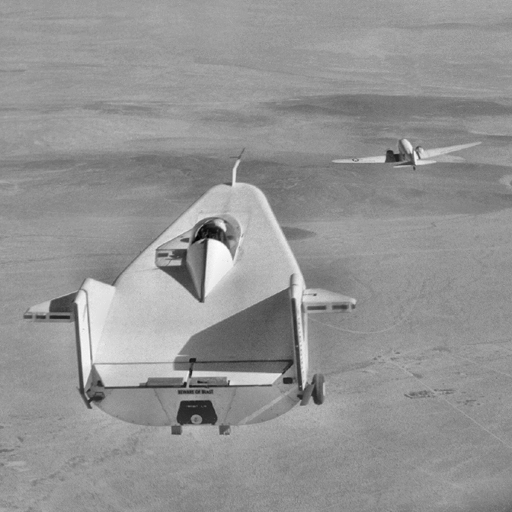
\includegraphics[width=\textwidth]{figure/1_tile_grid_size_12.png}
			\caption{滑动窗口边长=12}
		\end{subfigure}
		\begin{subfigure}[t]{\outwfour}
			\centering
			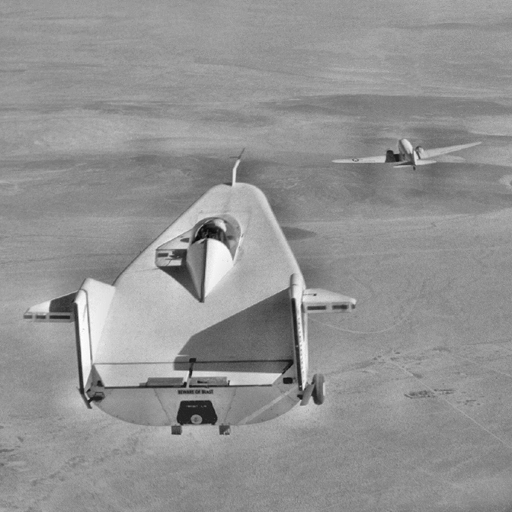
\includegraphics[width=\textwidth]{figure/1_tile_grid_size_16.png}
			\caption{滑动窗口边长=16}
		\end{subfigure}
		\caption{剪切限制为2、滑动窗口边长为4、8、12、16时的CLAHE处理结果}
		\label{fig:CLAHE3}
	\end{figure}
	可以看出,随着滑动窗口边长的增加,图像的局部对比度逐渐变得不均匀。当滑动窗口边长为4时图像CLAHE处理后具有更均匀的局部对比度。

	因此可以大致确定该图像最合适的CLAHE参数:剪切限制为2、滑动窗口边长为4。最终处理结果如图\ref{fig:CLAHE4}。
	\begin{figure}[htbp]
		\centering
		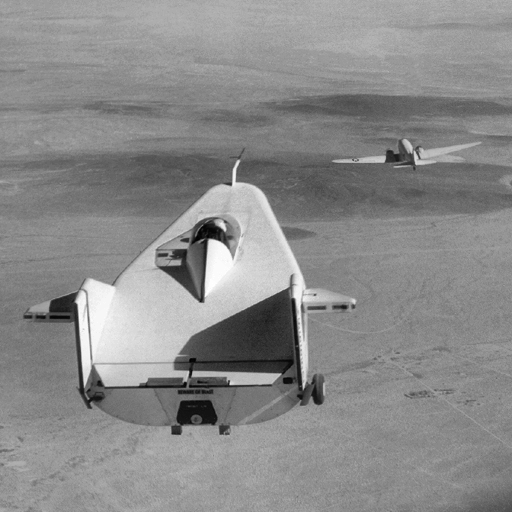
\includegraphics[width=0.5\textwidth]{figure/1_tile_grid_size_4.png}
		\caption{图\ref{pic:1}的最终处理结果}
		\label{fig:CLAHE4}
	\end{figure}

	\subsection{对图\ref{pic:2}的分析与图像增强}
	图\ref{pic:2}为一张X光图,属于医学影像图片,但图像主体中亮度不均,其中许多细节难以分辨,因此对图图\ref{pic:2}的处理应突出图像主体尽可能多的细节,以便于医生诊断。

	首先,图像主体亮度不均的问题可以通过同态滤波解决。选用Gaussian同态滤波器对图像进行处理,Gaussian同态滤波器传递函数$H(x,y)$为\cite{RN151}:
	\begin{equation}
		\begin{split}
			H(x,y)&=R_l+(R_h-R_l)\left(1-e^{-c(\frac{D(x,y)}{2d_0})^2}\right)\\
			D(x,y)&=\sqrt{(x-x_0)^2+(y-y_0)^2}
		\end{split}
	\end{equation}
	选取参数$R_l=0.5$、$R_h=4$、$c=3.5$、$d_0=3$\cite{RN151},对图像进行处理的结果如图\ref{fig:2homo}。
	\begin{figure}[htbp]
		\centering
		\begin{subfigure}[t]{\outwtwo}
			\centering
			\includegraphics[width=\textwidth]{figure/image2.jpg}
			\caption{原图}
		\end{subfigure}
		\begin{subfigure}[t]{\outwtwo}
			\centering
			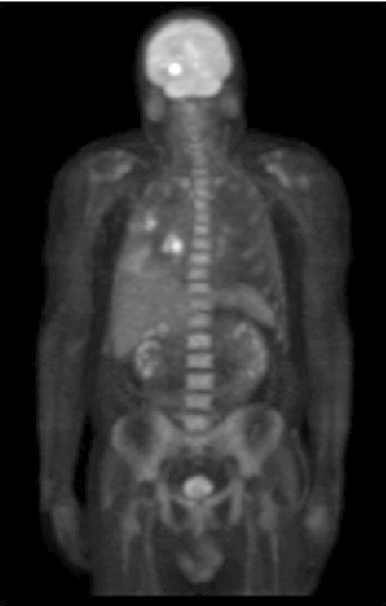
\includegraphics[width=\textwidth]{figure/2homo.png}
			\caption{同态滤波结果}
		\end{subfigure}
		\caption{图\ref{pic:2}的Gaussian同态滤波结果}
		\label{fig:2homo}
	\end{figure}[htbp]
	图中可以看出,Gaussian同态滤波使得图\ref{pic:2}中的很多细节得以显现,但图像整体对比度不高,需要进一步调整。

	为使得图像主体重要部位更容易辨认,可采用CLAHE对同态滤波后的图像进行直方图均衡化\cite{RN159},并采用同样的方法调节CLAHE的参数。首先固定滑动窗口边长为8,调节剪切限制为2、3、4、5,结果如图\ref{fig:2homoCLAHE_1}。可以看到剪切限制参数为3、4、5下的CLAHE操作均对图像有较好的对比度提升,但剪切限制为4、5时图像噪声较大,因此选择剪切限制为3进行进一步参数选择。
	\begin{figure}[htbp]
		\centering
		\begin{subfigure}[t]{\outwfour}
			\centering
			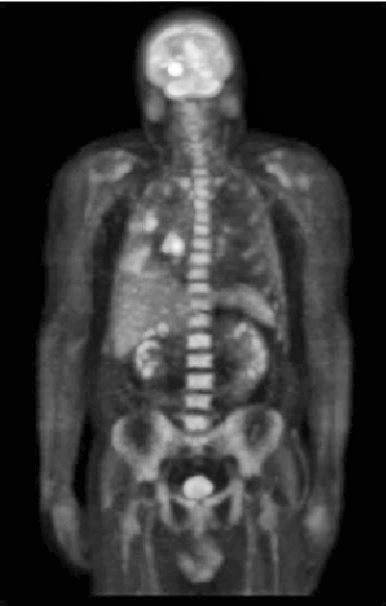
\includegraphics[width=\textwidth]{figure/2_clip_limit_2.png}
			\caption{剪切限制=2}
		\end{subfigure}
		\begin{subfigure}[t]{\outwfour}
			\centering
			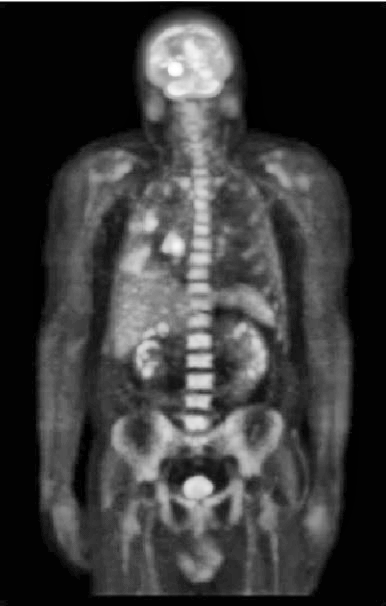
\includegraphics[width=\textwidth]{figure/2_clip_limit_3.png}
			\caption{剪切限制=3}
		\end{subfigure}
		\begin{subfigure}[t]{\outwfour}
			\centering
			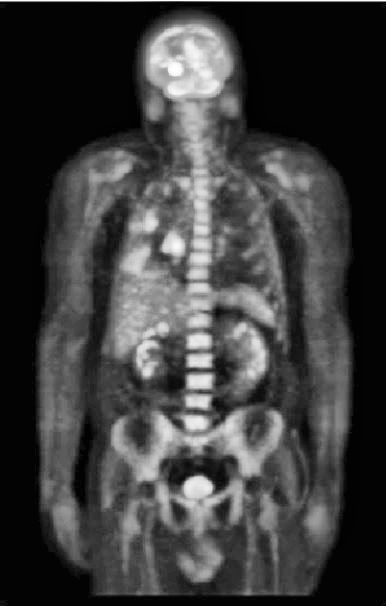
\includegraphics[width=\textwidth]{figure/2_clip_limit_4.png}
			\caption{剪切限制=4}
		\end{subfigure}
		\begin{subfigure}[t]{\outwfour}
			\centering
			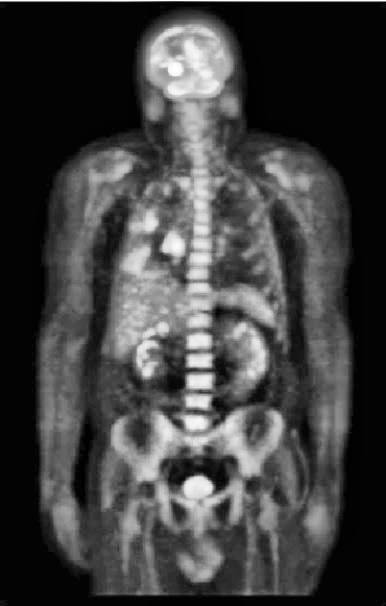
\includegraphics[width=\textwidth]{figure/2_clip_limit_5.png}
			\caption{剪切限制=5}
		\end{subfigure}
		\caption{剪切限制为2、3、4、5、滑动窗口边长为8时的CLAHE处理结果}
		\label{fig:2homoCLAHE_1}
	\end{figure}
	随后固定剪切限制为3调节滑动窗口边长为4、8、12、16,结果如图\ref{fig:2homoCLAHE_2}。可以看到在该图片中,滑动窗口边长对CLAHE的处理效果影响不大。但是随着滑动窗口边长的增加,图像中的重要部位更加突出,因此选择滑动窗口边长16作为CLAHE的调节参数。
	\begin{figure}[htbp]
		\centering
		\begin{subfigure}[t]{\outwfour}
			\centering
			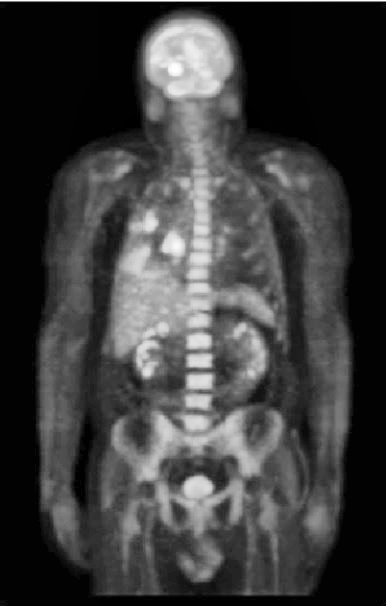
\includegraphics[width=\textwidth]{figure/2_tile_grid_size_4.png}
			\caption{滑动窗口边长=4}
		\end{subfigure}
		\begin{subfigure}[t]{\outwfour}
			\centering
			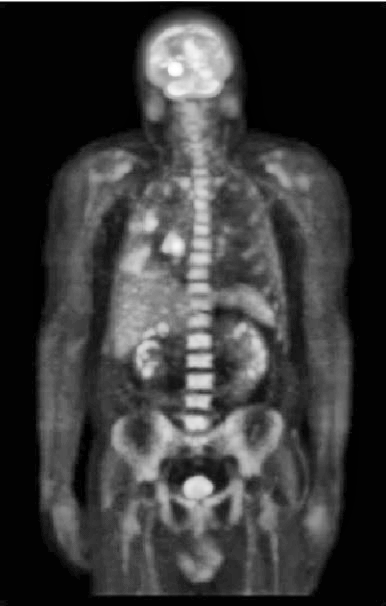
\includegraphics[width=\textwidth]{figure/2_tile_grid_size_8.png}
			\caption{滑动窗口边长=8}
		\end{subfigure}
		\begin{subfigure}[t]{\outwfour}
			\centering
			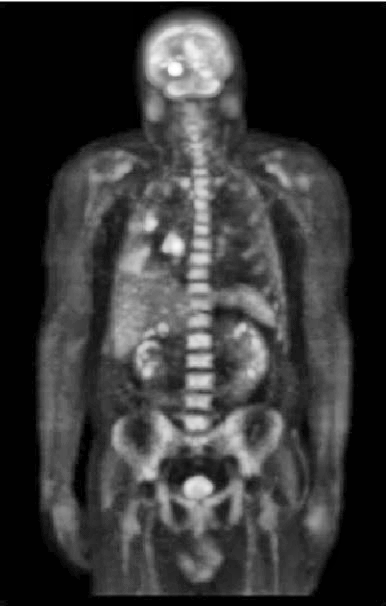
\includegraphics[width=\textwidth]{figure/2_tile_grid_size_12.png}
			\caption{滑动窗口边长=12}
		\end{subfigure}
		\begin{subfigure}[t]{\outwfour}
			\centering
			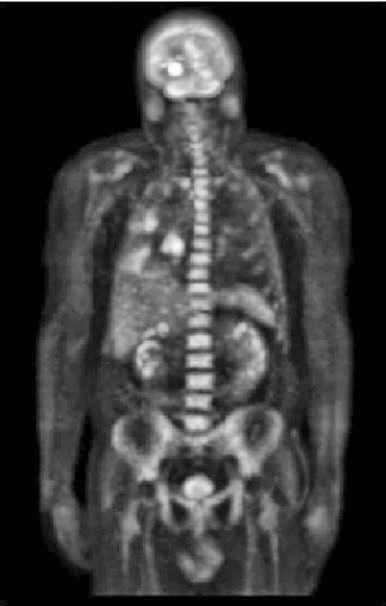
\includegraphics[width=\textwidth]{figure/2_tile_grid_size_16.png}
			\caption{滑动窗口边长=16}
		\end{subfigure}
		\caption{剪切限制为2、滑动窗口边长为4、8、12、16时的CLAHE处理结果}
		\label{fig:2homoCLAHE_2}
	\end{figure}
	综上,使用窗口边长为16、剪切限制为3的CLAHE对同态滤波后的图像进行进一步处理,得到最终处理结果如图\ref{fig:2homoCLAHE_3}。
	\begin{figure}[htbp]
		\centering
		\begin{subfigure}[t]{\outwthree}
			\centering
			\includegraphics[width=\textwidth]{figure/image2.jpg}
			\caption{原图}
		\end{subfigure}
		\begin{subfigure}[t]{\outwthree}
			\centering
			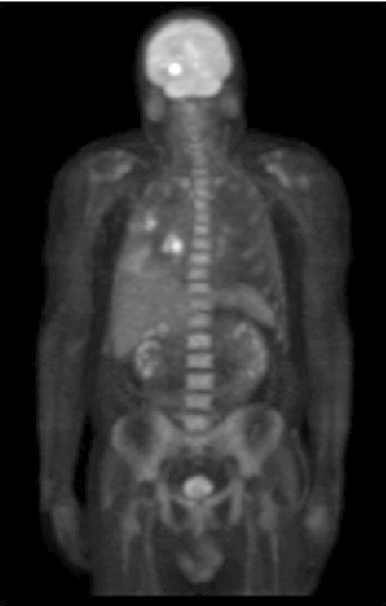
\includegraphics[width=\textwidth]{figure/2homo.png}
			\caption{同态滤波结果}
		\end{subfigure}
		\begin{subfigure}[t]{\outwthree}
			\centering
			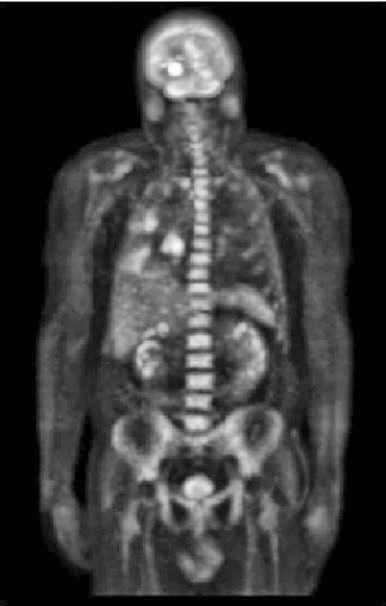
\includegraphics[width=\textwidth]{figure/2_tile_grid_size_16.png}
			\caption{CLAHE结果}
		\end{subfigure}
		\caption{图\ref{pic:2}的最终处理结果}
		\label{fig:2homoCLAHE_3}
	\end{figure}

	\subsection{对图\ref{pic:3}的分析与图像增强}
	首先从图\ref{pic:3}中可以直观的看出,该图中有很强的椒盐噪声,应先使用中值滤波器进行降噪。采用核边长为3的中值滤波器对图像进行滤波,结果如图\ref{fig:3blur}可以看到图像的椒盐噪声被有效地去除了。
	\begin{figure}[htbp]
		\centering
		\begin{subfigure}[t]{\outwtwo}
			\centering
			\includegraphics[width=\textwidth]{figure/image3.jpg}
			\caption{原图}
		\end{subfigure}
		\begin{subfigure}[t]{\outwtwo}
			\centering
			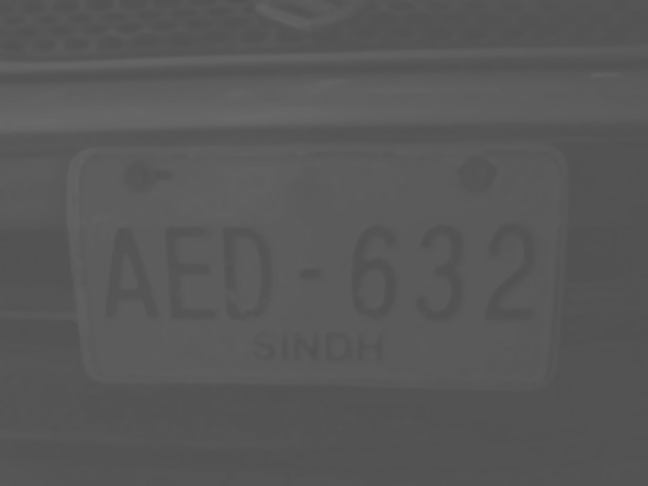
\includegraphics[width=\textwidth]{figure/3_img_blur.png}
			\caption{中值滤波结果}
		\end{subfigure}
		\caption{图\ref{pic:3}的中值滤波处理结果}
		\label{fig:3blur}
	\end{figure}
	椒盐噪声去除后,进一步绘制图像的灰度直方图,如图\ref{fig:3blur_hist}。
	\begin{figure}[htbp]
		\centering
		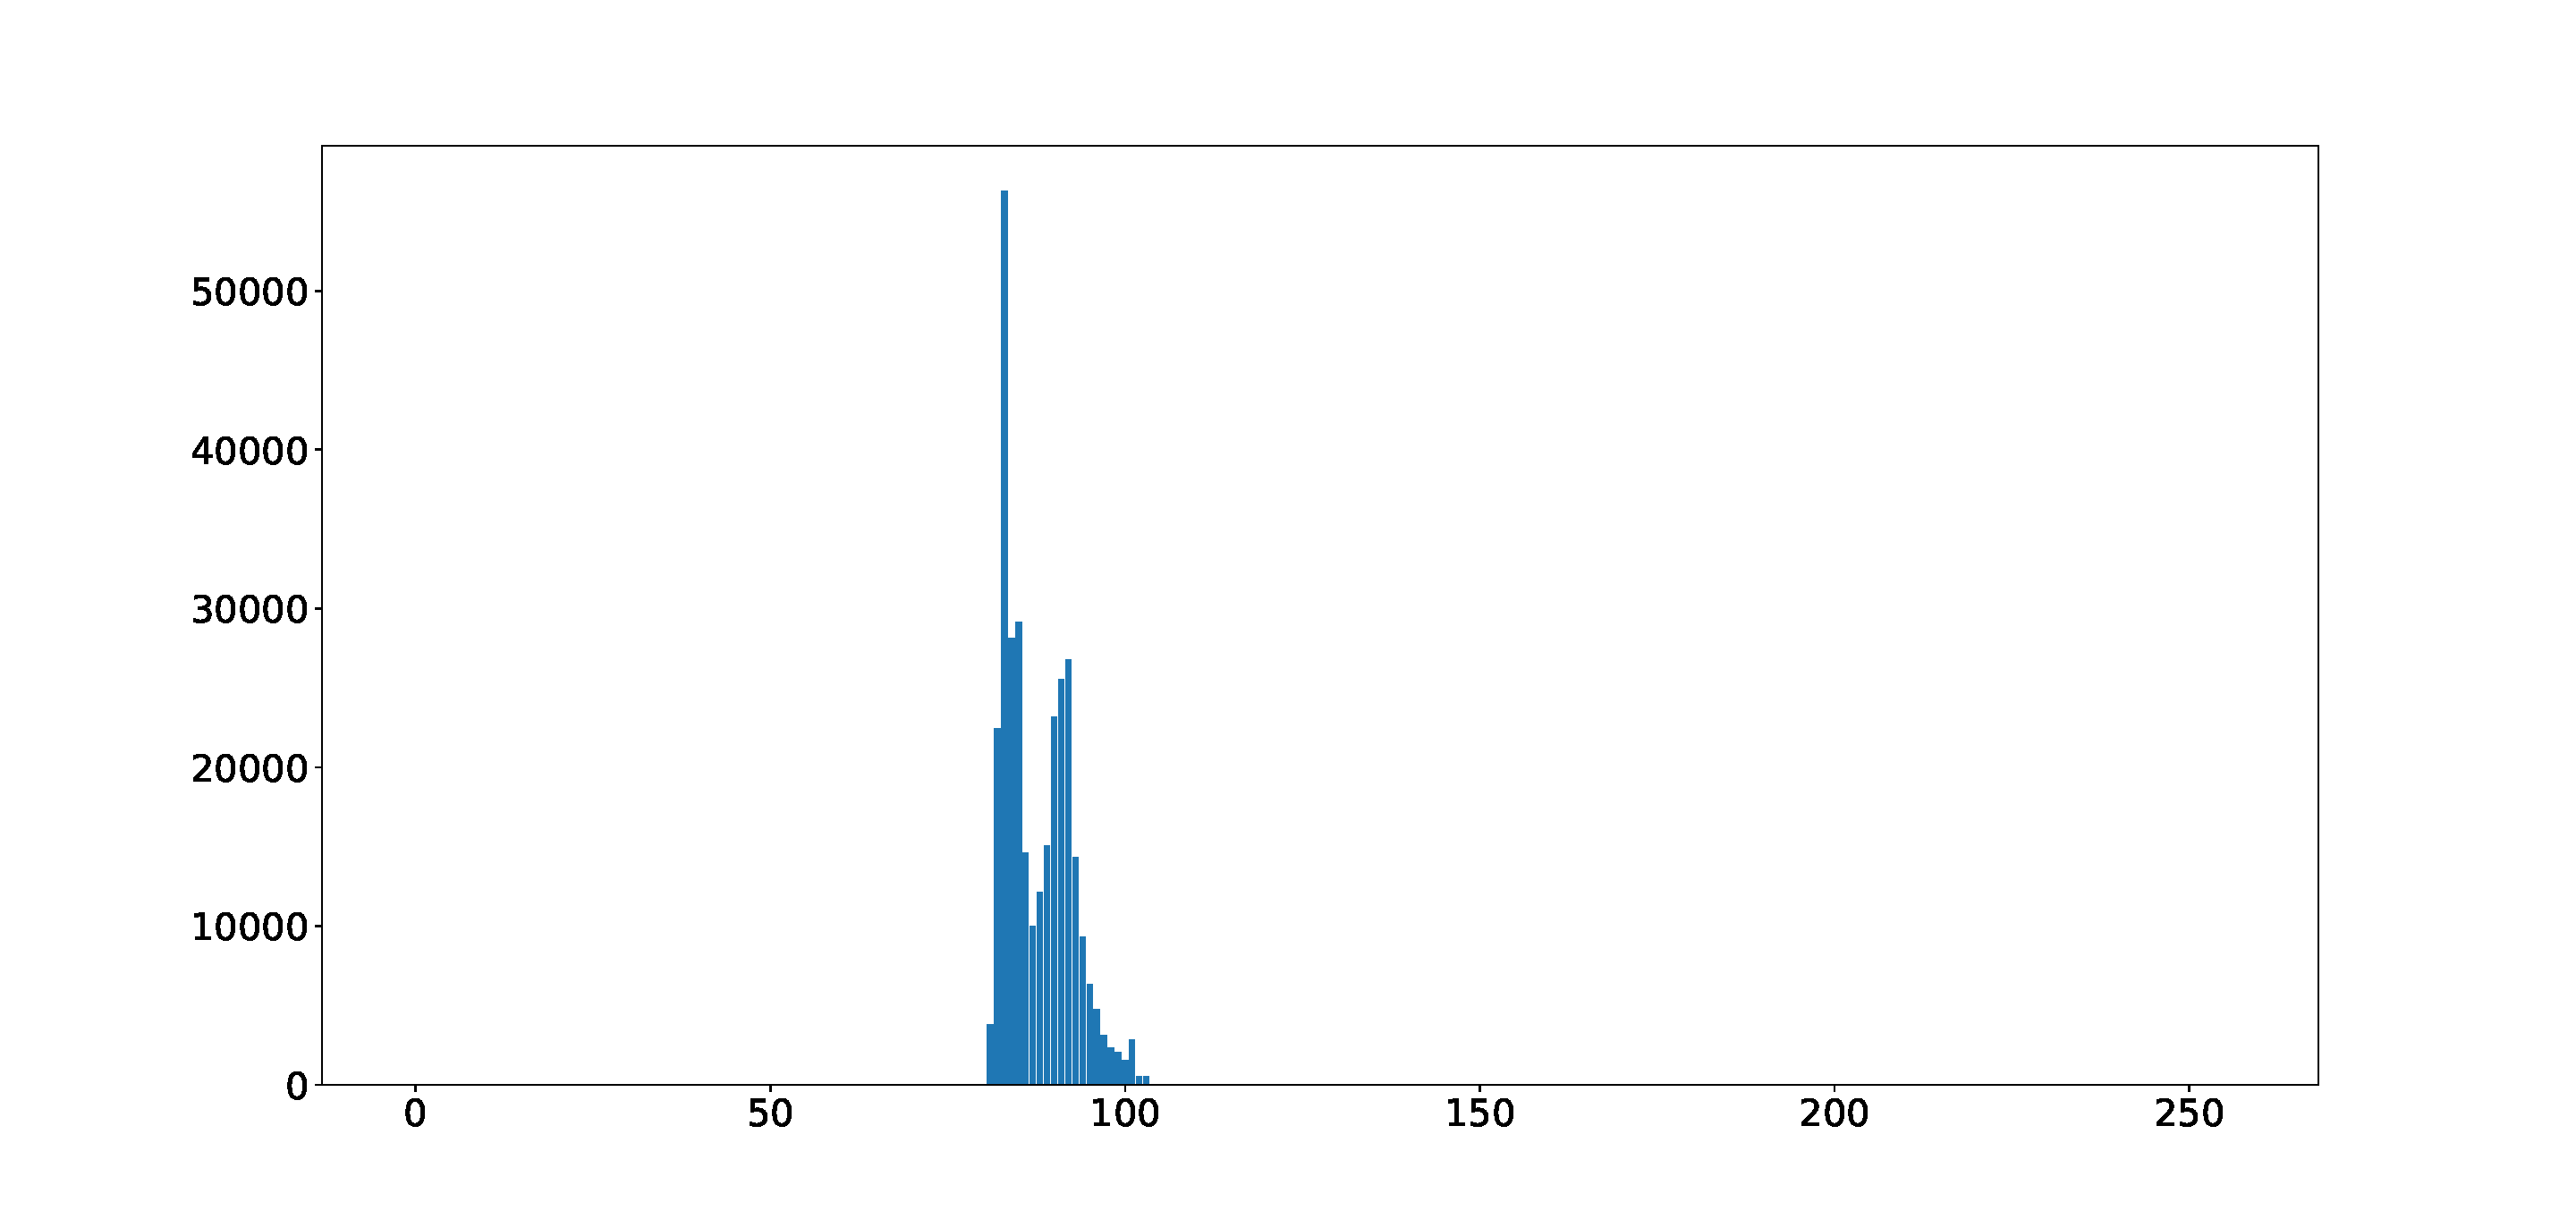
\includegraphics[width=\textwidth]{figure/3_img_blur_hist.pdf}
		\caption{图\ref{pic:3}经过中值滤波处理结果的灰度直方图}
		\label{fig:3blur_hist}
	\end{figure}
	从图中可以看出,经过中值滤波处理后的图\ref{pic:3}存在严重的灰度不均的问题,需要进行直方图均衡化。采用\ref{sec:处理1}节中的CLAHE方法和参数对经过中值滤波处理后的图\ref{pic:3}进行直方图均衡化,结果如图\ref{fig:3blur_clahe}。
	\begin{figure}[htbp]
		\centering
		\begin{subfigure}[t]{\outwtwo}
			\centering
			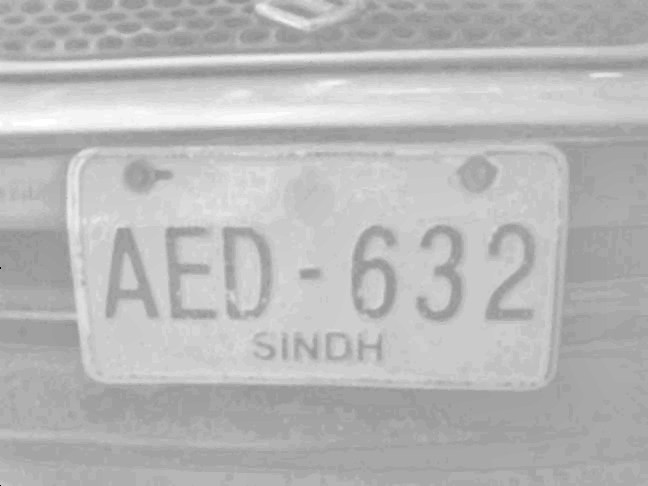
\includegraphics[width=1.05\textwidth]{figure/3_img_clahe_1.png}
			\caption{直方图均衡化处理结果}
		\end{subfigure}
		\begin{subfigure}[t]{\outwtwo}
			\centering
			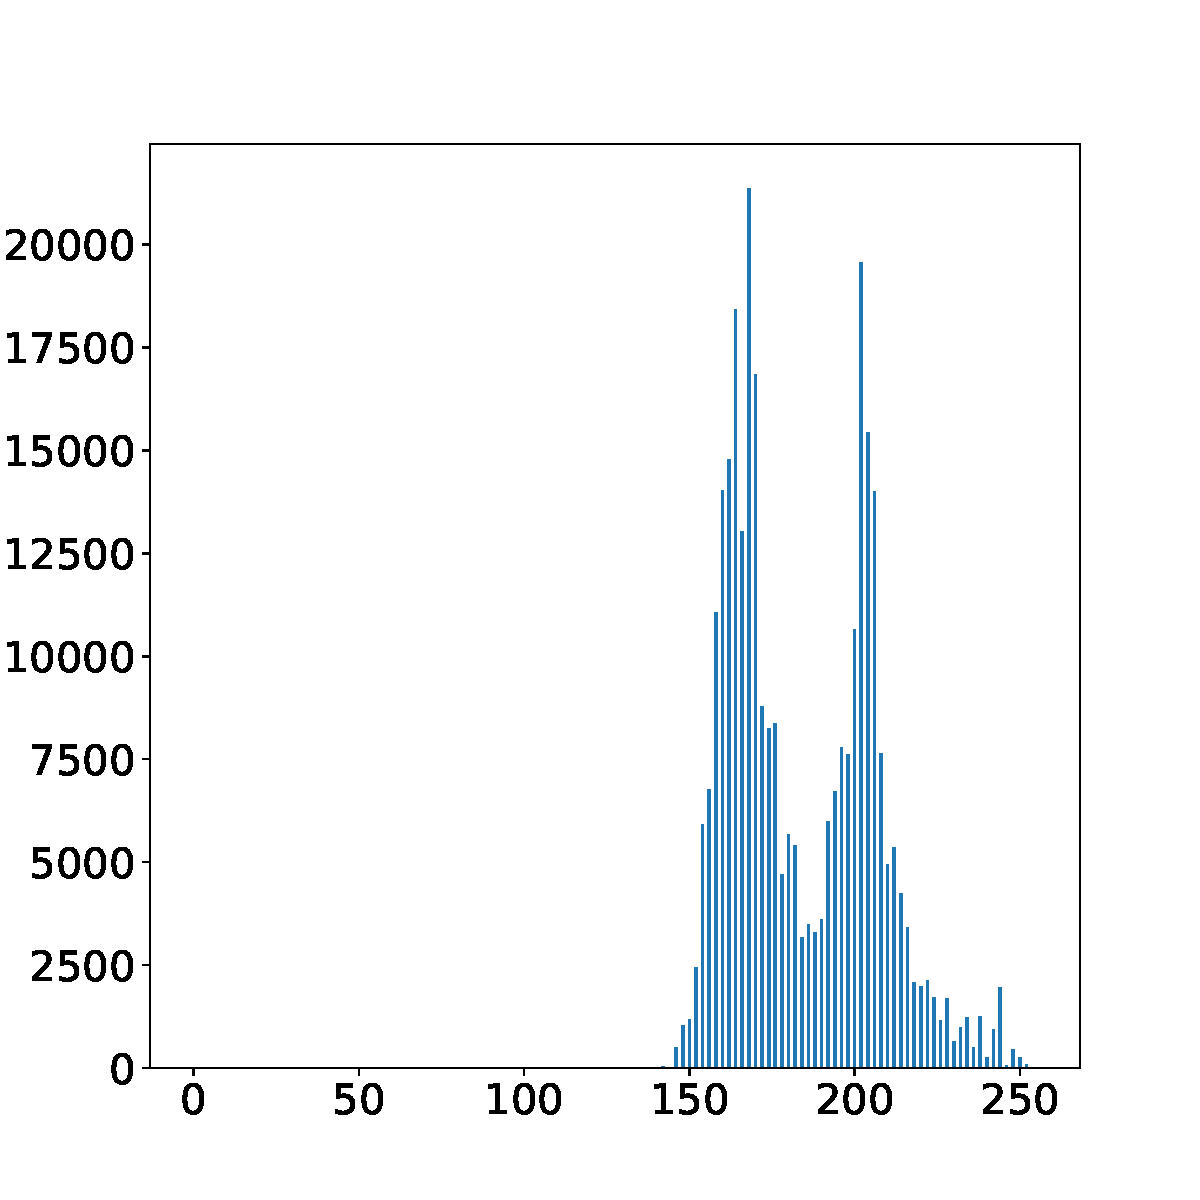
\includegraphics[width=0.87\textwidth]{figure/3_img_clahe_1.pdf}
			\caption{处理后的灰度直方图}
		\end{subfigure}
		\caption{图\ref{pic:3}中值滤波处理后CLAHE处理结果}
		\label{fig:3blur_clahe}
	\end{figure}
	从图中可以看出,CLAHE的处理效果并不理想,图像中大部分像素的灰度都被压缩到一个较高的值。查阅文献可知,这个现象是由于图像中存在灰度值和大部分像素相差较远的“离群像素”导致,在进行CLAHE前需要将这些像素剔除\cite{RN154}。

	进一步计算可以发现,在整张图片中,除了3个灰度值为0的像素外,其余像素的灰度取值范围均为$\left[80,104\right]$,图像中确实存在3个“离群像素”。将这三个离群像素的灰度值修改为80,使用同样参数再次进行CLAHE操作,结果如图\ref{fig:3blur_clahe_2}。
	\begin{figure}[htbp]
		\centering
		\begin{subfigure}[t]{\outwtwo}
			\centering
			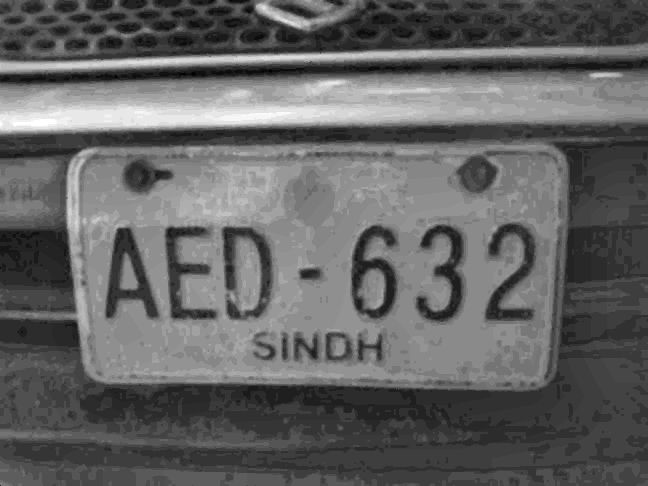
\includegraphics[width=1.05\textwidth]{figure/3_img_clahe_2.png}
			\caption{直方图均衡化处理结果}
		\end{subfigure}
		\begin{subfigure}[t]{\outwtwo}
			\centering
			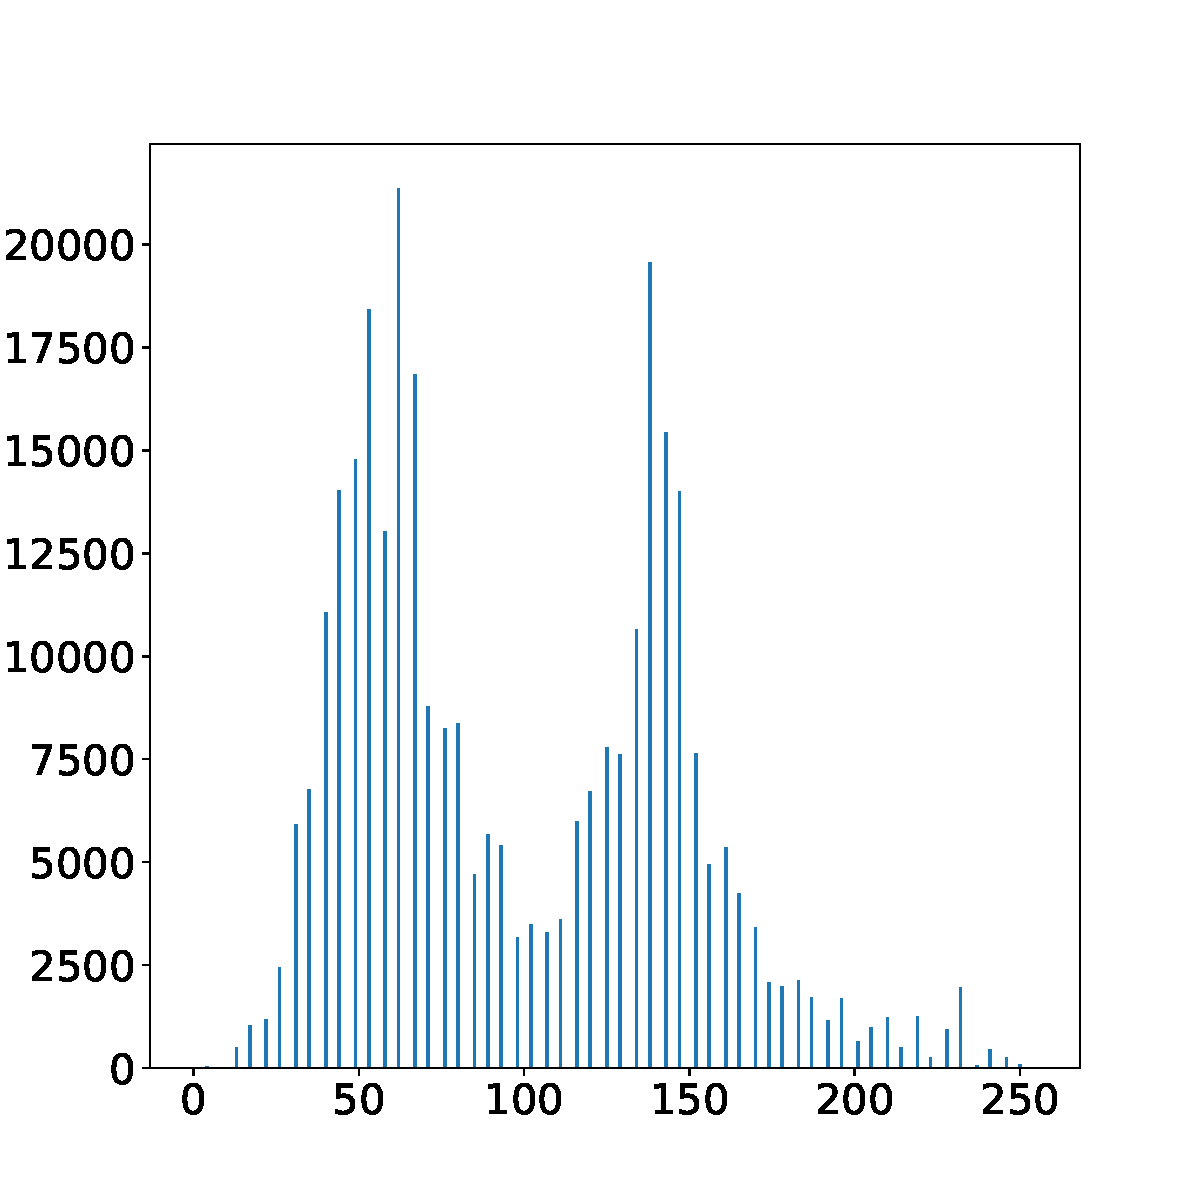
\includegraphics[width=0.87\textwidth]{figure/3_img_clahe_2.pdf}
			\caption{处理后的灰度直方图}
		\end{subfigure}
		\caption{剔除离群像素后CLAHE处理结果}
		\label{fig:3blur_clahe_2}
	\end{figure}
	可以看出,剔除离群像素后,CLAHE处理效果有明显提升,图片中像素灰度分布更加均匀。因此以图\ref{fig:3blur_clahe_2}作为图\ref{pic:3}的图像增强结果,进行进一步的形态学分析。

	\subsection{图\ref{pic:3}的形态学分析与提取有用信息区域}
	完成对图\ref{pic:3}的图像增强操作后,对增强结果进行形态学分析。首先确定灰度范围对图像进行二值化处理。先设定灰度下限为0,调节灰度上限,对图像进行二值化操作,结果如图\ref{fig:3mask_1}。
	\begin{figure}[htbp]
		\centering
		\begin{subfigure}[t]{\outwfour}
			\centering
			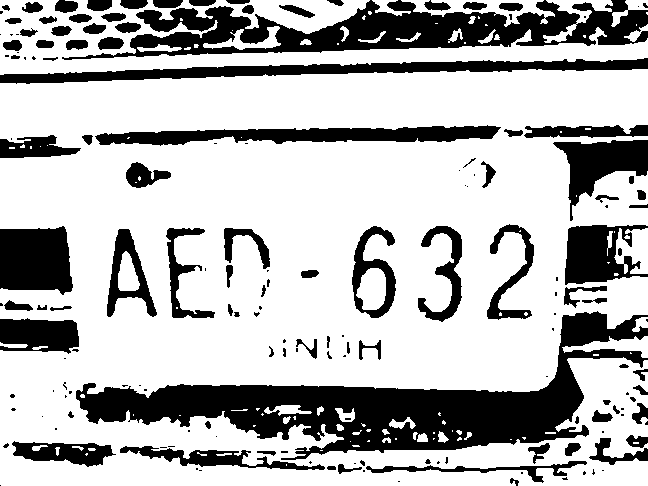
\includegraphics[width=\textwidth]{figure/3mask_1_1.png}
			\caption{灰度上限=60}
		\end{subfigure}
		\begin{subfigure}[t]{\outwfour}
			\centering
			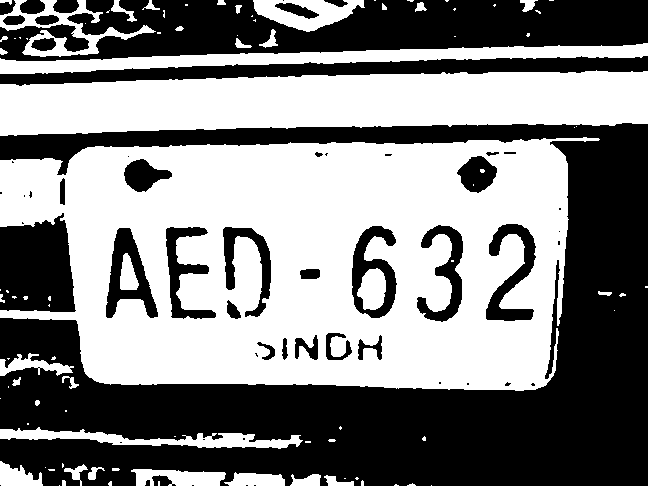
\includegraphics[width=\textwidth]{figure/3mask_1_2.png}
			\caption{灰度上限=80}
		\end{subfigure}
		\begin{subfigure}[t]{\outwfour}
			\centering
			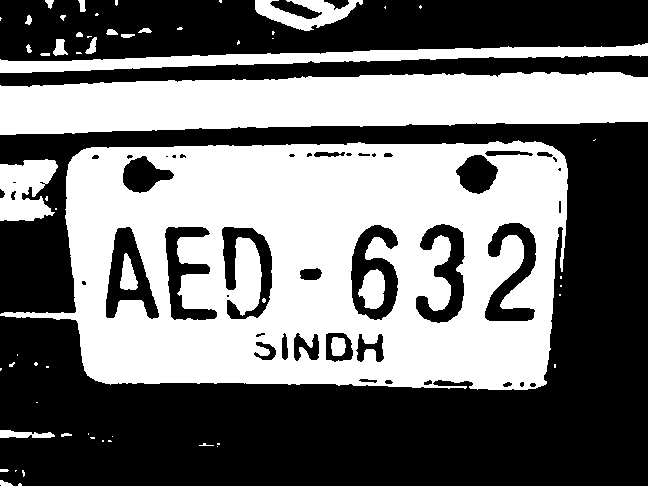
\includegraphics[width=\textwidth]{figure/3mask_1_3.png}
			\caption{灰度上限=100}
		\end{subfigure}
		\begin{subfigure}[t]{\outwfour}
			\centering
			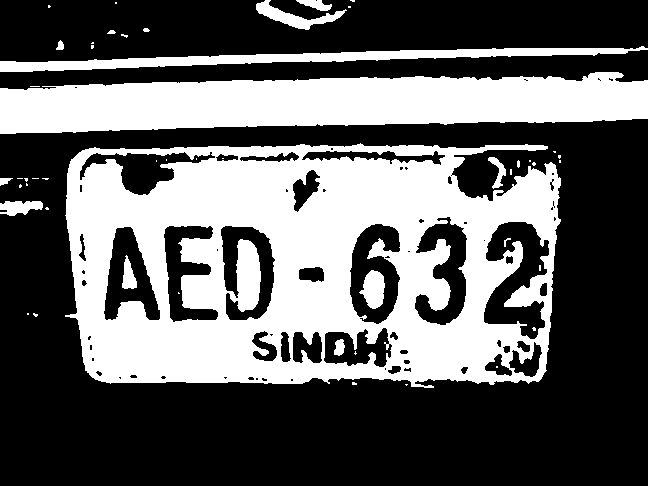
\includegraphics[width=\textwidth]{figure/3mask_1_4.png}
			\caption{灰度上限=120}
		\end{subfigure}
		\caption{灰度下限为0、灰度上限为60、80、100、120时的图像二值化处理结果}
		\label{fig:3mask_1}
	\end{figure}
	可以看到,随着灰度范围上限的上升,图像主体部分的轮廓趋于完整,而当灰度上限达到120时,许多不属于图像主体的部分对图像主体的轮廓产生了干扰。因此选择使图像主体较为完整且干扰较少的灰度上限100,进行后续调整。

	进一步固定灰度上限,调整灰度下限对图像进行二值化操作。结果如图\ref{fig:3mask_2}。
	\begin{figure}[htbp]
		\centering
		\begin{subfigure}[t]{\outwfour}
			\centering
			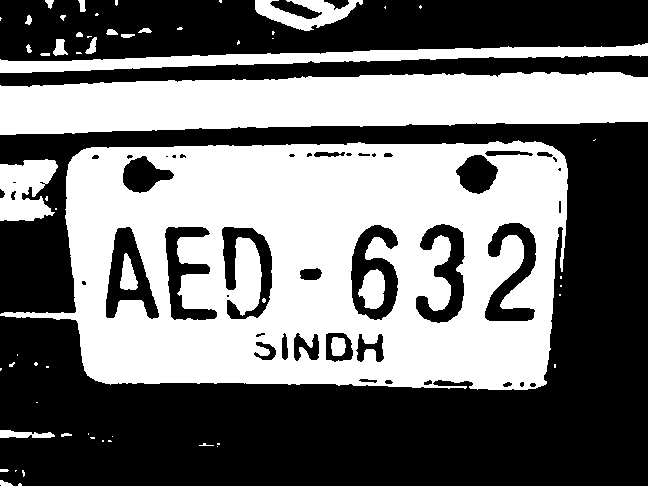
\includegraphics[width=\textwidth]{figure/3mask_2_1.png}
			\caption{灰度下限=0}
		\end{subfigure}
		\begin{subfigure}[t]{\outwfour}
			\centering
			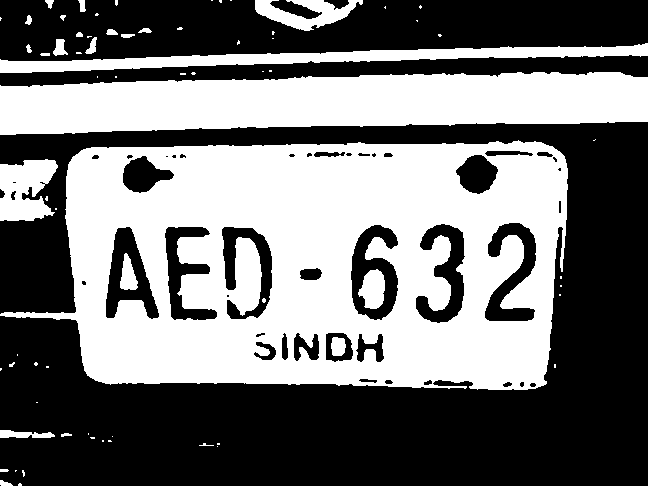
\includegraphics[width=\textwidth]{figure/3mask_2_2.png}
			\caption{灰度下限=10}
		\end{subfigure}
		\begin{subfigure}[t]{\outwfour}
			\centering
			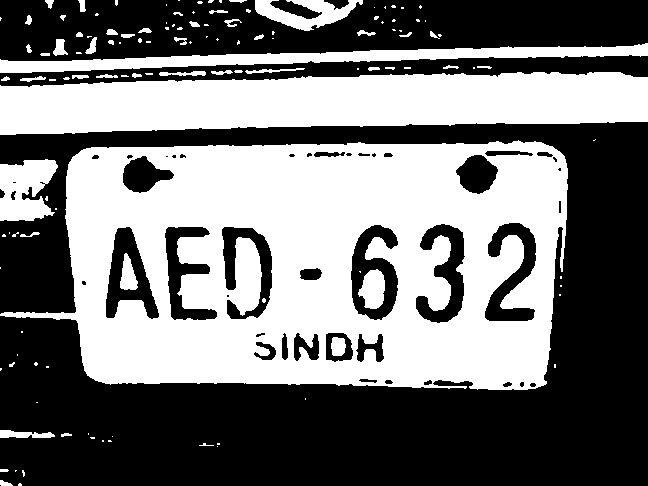
\includegraphics[width=\textwidth]{figure/3mask_2_3.png}
			\caption{灰度下限=20}
		\end{subfigure}
		\begin{subfigure}[t]{\outwfour}
			\centering
			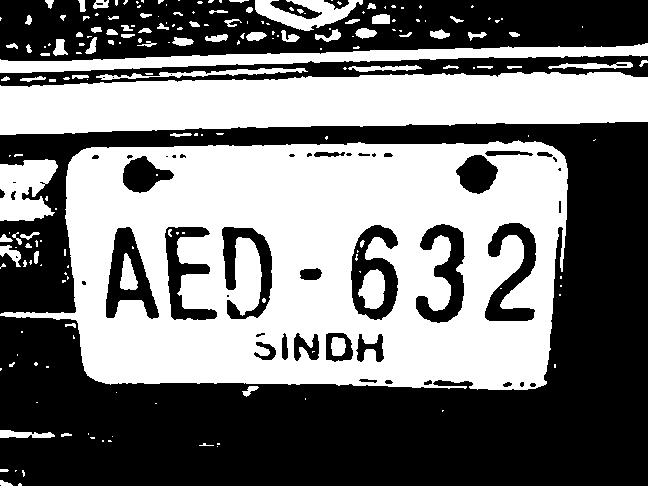
\includegraphics[width=\textwidth]{figure/3mask_2_4.png}
			\caption{灰度下限=30}
		\end{subfigure}
		\caption{灰度下限为0、10、20、30、灰度上限为100时的图像二值化处理结果}
		\label{fig:3mask_2}
	\end{figure}
	可以看出,随着灰度下限的上升,二值图像中出现了越来越多的非主体部分的细节,且图像主体部分随之出现了部分残缺。因此二值化灰度下限应选择最能突出图像主体的0灰度下限。故确定二值化的灰度选择范围为$\left[0,100\right]$。最终二值图像如图\ref{fig:3mask}。
	\begin{figure}[htbp]
		\centering
		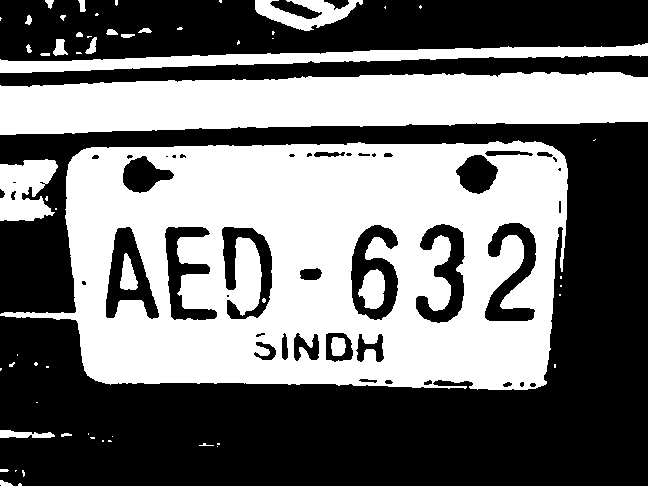
\includegraphics[width=0.8\textwidth]{figure/3mask_2_1.png}
		\caption{图\ref{pic:3}的二值图像}\label{fig:3mask}
	\end{figure}

	对二值图像(图\ref{fig:3mask}),图像主体的内容为车辆牌照,其有用信息区域为中央数字和字母区域。一般车辆牌照的文字有统一的大小、牌照字符和牌照背景有较大的对比度,因此在识别车牌灰度图像时可以考虑使用在水平和垂直方向上进行一阶差分运算后再进行累加,以统计出灰度变化频繁的区域\cite{RN160}。水平方向一阶差分的算式为:
	\begin{equation}
		\begin{split}
			G_w(i)&=\sum_{j=0}^wg(i,j)\\
			g_w(i,j)&=|f(i,j)-f(i,j+1)|
		\end{split}
	\end{equation}
	垂直方向一阶差分的算式为:
	\begin{equation}
		\begin{split}
			G_h(j)&=\sum_{i=0}^hg(i,j)\\
			g_h(i,j)&=|f(i,j)-f(i+1,j)|
		\end{split}
	\end{equation}
	其中$(i,j)$为图像中的像素点,$w$和$h$为图像宽度和高度,$g_w(i,j)$和$g_h(i,j)$分别为水平和垂直差分图像,$G(i)$和$G(i)$分别为水平和垂直方向的累加结果,$f(i,j)$为像素点灰度值或是二值化图像中的01值。此外,在二值化图像中,由于字符只占牌照背景的一小部分,因此可以在一阶差分运算累加前通过一个较大的核对二值图像进行形态学闭运算以抹去图像中非牌照部分的对比度从而提高识别准确率\cite{RN161}。此处选用一个12$\times$12的方形核对图像进行一次形态学闭运算,再统计水平和垂直方向上的差分累加结果,可得图\ref{fig:3ghist}。
	\begin{figure}[htbp]
		\centering
		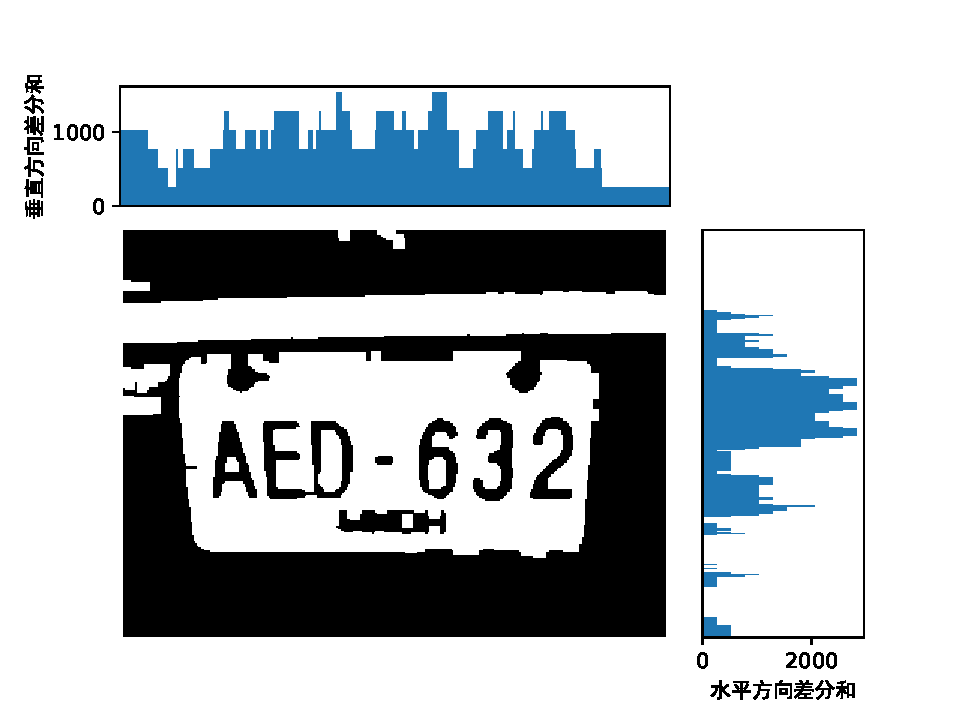
\includegraphics[width=\textwidth]{figure/3Ghist.pdf}
		\caption{闭运算及差分累加结果}\label{fig:3ghist}
	\end{figure}
	由图可知在水平方向的差分累加结果差异更加显著,因此可以先进行垂直方向的图像范围确定。从水平方向差分累加图中选出结果较大区域,可以得到垂直方向上的有用图像范围为$\left[145,391\right]$,以此范围对图像进行裁剪,并再次计算垂直方向差分累加,结果如图\ref{fig:3ghist1}。
	\begin{figure}[htbp]
		\centering
		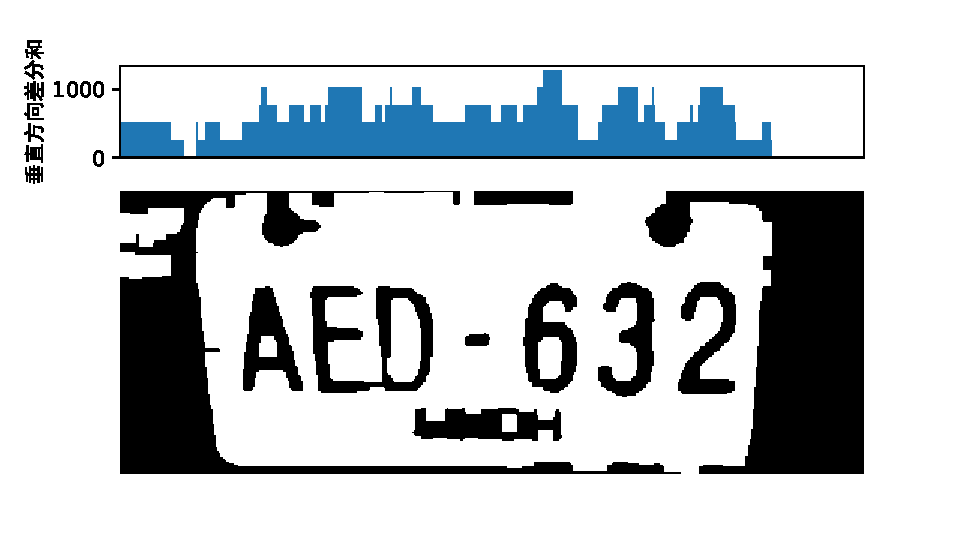
\includegraphics[width=\textwidth]{figure/3Ghist1.pdf}
		\caption{裁剪及垂直方向差分累加结果}\label{fig:3ghist1}
	\end{figure}
	从垂直方向差分累加图中选出结果较大区域,可以得到水平方向上的有用图像范围为$\left[67,568\right]$。

	综上,由形态学分析得出的车牌照有用信息的像素范围为水平方向$\left[67,568\right]$和垂直方向$\left[67,568\right]$。在图\ref{fig:3mask}上对此范围内的图像区域进行裁剪,结果如图\ref{fig:3maskcut}。
	\begin{figure}[htbp]
		\centering
		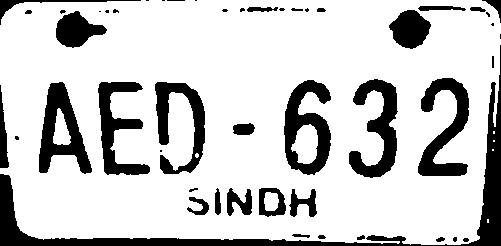
\includegraphics[width=\textwidth]{figure/3maskcut.png}
		\caption{车牌范围裁剪结果}\label{fig:3maskcut}
	\end{figure}

	确定了车牌照有用信息的像素范围后即可进一步通过连通域确定车牌数字的具体位置。调用opencv中的cv2.findContours()函数查找图\ref{fig:3maskcut}中的连通域,除去最外层的连通边框,选择剩余连通域中面积最大的15个连通域,调用cv2.drawContours()函数将这些连通域标出,得到图\ref{fig:3maskcutsel}。
	\begin{figure}[htbp]
		\centering
		\includegraphics[width=\textwidth]{figure/3maskcut_sel.png}
		\caption{连通域选择与标记结果}\label{fig:3maskcutsel}
	\end{figure}
	可以看出,虽然数字和字母位置都能被准确标出,但有部分标记在非数字和字母位置,标记效果有待提升。

	\subsection{对图\ref{pic:4}的分析与图像增强}
	从图\ref{pic:4}中可以看到明显的动态模糊,需要对图像进行去模糊处理。依照实验指导中已经给出的降质函数假设$len=8,\theta=0$,图像模糊为水平方向平移模糊8像素。因此分别采用维纳滤波、可约束最小二乘滤波和Lucy-Richardson滤波三种方法对图像进行滤波处理并进行对比,结果如图\ref{fig:4filter}。
	\begin{figure}[htbp]
		\centering
		\includegraphics[width=0.8\textwidth]{figure/4filter.pdf}
		\caption{三种滤波方法对比}\label{fig:4filter}
	\end{figure}
	可以看出在默认参数情况下,Lucy-Richardson滤波效果最好,可约束最小二乘滤波其次,而维纳滤波效果最差。

	在可约束最小二乘滤方法和维纳滤波方法中,都需要估计图像的信噪比(SNR)或者噪声功率,信号的功率谱使用图像的方差近似估计,使得噪声分布已知。因此可以通过调节滤波器的噪声参数调整图像的处理效果。

	分别假定图像的噪声功率为0、0.01、1、100,使用可约束最小二乘滤波器对图像进行处理,结果如图\ref{fig:4reg}。
	\begin{figure}[htbp]
		\centering
		\begin{subfigure}[t]{\outwfour}
			\centering
			\includegraphics[width=\textwidth]{figure/deconvreg1.png}
			\caption{噪声功率为0}
		\end{subfigure}
		\begin{subfigure}[t]{\outwfour}
			\centering
			\includegraphics[width=\textwidth]{figure/deconvreg2.png}
			\caption{噪声功率为0.01}
		\end{subfigure}
		\begin{subfigure}[t]{\outwfour}
			\centering
			\includegraphics[width=\textwidth]{figure/deconvreg3.png}
			\caption{噪声功率为1}
		\end{subfigure}
		\begin{subfigure}[t]{\outwfour}
			\centering
			\includegraphics[width=\textwidth]{figure/deconvreg4.png}
			\caption{噪声功率为100}
		\end{subfigure}
		\caption{噪声功率为0、0.01、1、100时的可约束最小二乘滤波结果}
		\label{fig:4reg}
	\end{figure}
	从图中可以看出,假设了噪声功率的可约束最小二乘滤波器对图像的恢复能力有所提升,而当假定噪声功率增大时,图像又趋于模糊。可以得到该图的较好的可约束最小二乘滤波噪声功率大致在0.01$\sim$100之间。

	分别假定图像的信噪比为0、0.01、0.1、1,使用维纳滤波器对图像进行处理,结果如图\ref{fig:4wnr}。
	\begin{figure}[htbp]
		\centering
		\begin{subfigure}[t]{\outwfour}
			\centering
			\includegraphics[width=\textwidth]{figure/deconvwnr1.png}
			\caption{信噪比为0}
		\end{subfigure}
		\begin{subfigure}[t]{\outwfour}
			\centering
			\includegraphics[width=\textwidth]{figure/deconvwnr2.png}
			\caption{信噪比为0.01}
		\end{subfigure}
		\begin{subfigure}[t]{\outwfour}
			\centering
			\includegraphics[width=\textwidth]{figure/deconvwnr3.png}
			\caption{信噪比为0.1}
		\end{subfigure}
		\begin{subfigure}[t]{\outwfour}
			\centering
			\includegraphics[width=\textwidth]{figure/deconvwnr4.png}
			\caption{信噪比为1}
		\end{subfigure}
		\caption{信噪比为0、0.01、0.1、1时的图像维纳滤波结果}
		\label{fig:4wnr}
	\end{figure}
	从图中可以看出,假设了信噪比的维纳滤波器对图像的恢复能力有明显提升,而当假定信噪比增大时,图像又趋于模糊且整体变暗。可以得到该图的较好的维纳滤波信噪比大致在0.01$\sim$0.1之间。

	\section{实验结果及讨论}
	\subsection{实验结果}
	\begin{enumerate}
		\item 在对图\ref{pic:1}的分析与处理中,本文使用了标准直方图均衡化和自适应直方图均衡化两种方法对原始图像进行了处理,发现了标准直方图均衡化在处理灰度分布严重不均的图片时存在的问题;同时通过各种参数的组合尝试与对比大致确定了对该图像进行图像增强时最合适的CLAHE参数,并给出了最终的处理结果图\ref{fig:CLAHE4};
		\item 在对图\ref{pic:2}的分析与处理中,本文首先使用了Gaussian同态滤波对图像各区域亮度进行了均衡,随后在均衡亮度的基础上使用了和处理图\ref{pic:1}类似的方法选择CLAHE参数对图像的对比度进行了增强,最终处理结果如图\ref{fig:2homoCLAHE_3};
		\item 在对图\ref{pic:3}的分析与处理中,本文首先使用中值滤波器对图像中的椒盐噪声进行了处理,随后在使用CLAHE方法进行对比度增强时发现图像中的少数离群像素导致增强效果不佳,并使用非离群像素点的最小灰度代替了离群像素点位置的灰度值,获得了较好的CLAHE处理效果,结果如图\ref{fig:3blur_clahe_2};
		\item 在提取图\ref{pic:3}中的有用信息区域时,本文首先通过尝试和对比确定了一个合适的二值化灰度范围,获得二值图像后,首先对二值图像进行了一次闭运算抹去图像有用信息区域外的大部分轮廓,随后采用统计水平和垂直方向上的像素差分累加和的方法确定了有用信息区域的大致范围,最后使用连通域选择方法找出了图像中的有用信息,结果如图\ref{fig:3maskcutsel};
		\item 在对图\ref{pic:3}的分析与处理中,本文首先采用三种滤波方法使用默认设置对图像进行处理并对比了处理结果(图\ref{fig:4filter}),随后通过调节信噪比参数和噪声功率参数调节了其中两种滤波方法,并对其结果(图\ref{fig:4reg}、\ref{fig:4wnr})进行了对比。
	\end{enumerate}

	\subsection{讨论}
	\begin{enumerate}
		\item 从对图\ref{pic:1}、图\ref{pic:2}和图\ref{pic:3}的处理过程中可以发现,对于CLAHE方法,不同的图像各自有其适合的参数,且对于存在离群像素的图片,CLAHE方法并不能很好的发挥效果;
		\item 从对图\ref{pic:2}的处理过程中可以发现,同态滤波虽然能够修复图像亮度不均的问题,却会导致图像出现对比度下降,在X影像增强时需要辅以对比度增强的方法才能获得较好的处理效果;
		\item 在对图\ref{pic:3}的处理过程中,本文采用了先确定有用信息大致范围再使用连通域判断的方法,能一定程度上避免有用区域外和有用区域中的形态相近的区域的影响;
		\item 从对图\ref{pic:4}的处理过程中可以发现,调节先验的噪声参数会对可约束最小二乘滤波和维纳滤波的效果产生很大影响,在实际应用中应按照实际使用设备中的噪声情况选择合适的参数。
	\end{enumerate}

	\bibliography{ref}
	\bibliographystyle{unsrt}
\end{spacing}
\end{document}